% !TeX spellcheck = de_DE
\documentclass{article}

\usepackage[ngerman]{babel}
\usepackage{graphicx}
\usepackage{indentfirst}
\usepackage{hyperref}
\usepackage{geometry}
\usepackage{changepage}

\graphicspath{ {./images/} }

\makeatletter
\newcommand{\sectionauthor}[1]{
	{\parindent 0em \large \scshape Autor: #1 \par \nobreak \vspace*{1em}}
	\@afterheading
}
\newcommand{\specification}[3]{
	{\parindent 0.5em \hangindent 3em \hypertarget{spec:#1:#2}{\textbf{/#1#2/}} #3 \par \nobreak \vspace*{0.5em}}
}
\makeatother

\title{Bibliothekanwendung - Pflichtenheft}
\date{\today}
\author{
	Ivan Charviakou\\
	León Liehr\\
	Mohamad Najjar\\
	Jonas Picker\\
	Sergei Pravdin
}

\begin{document}

\maketitle
\begin{figure}[h]
	\centering
	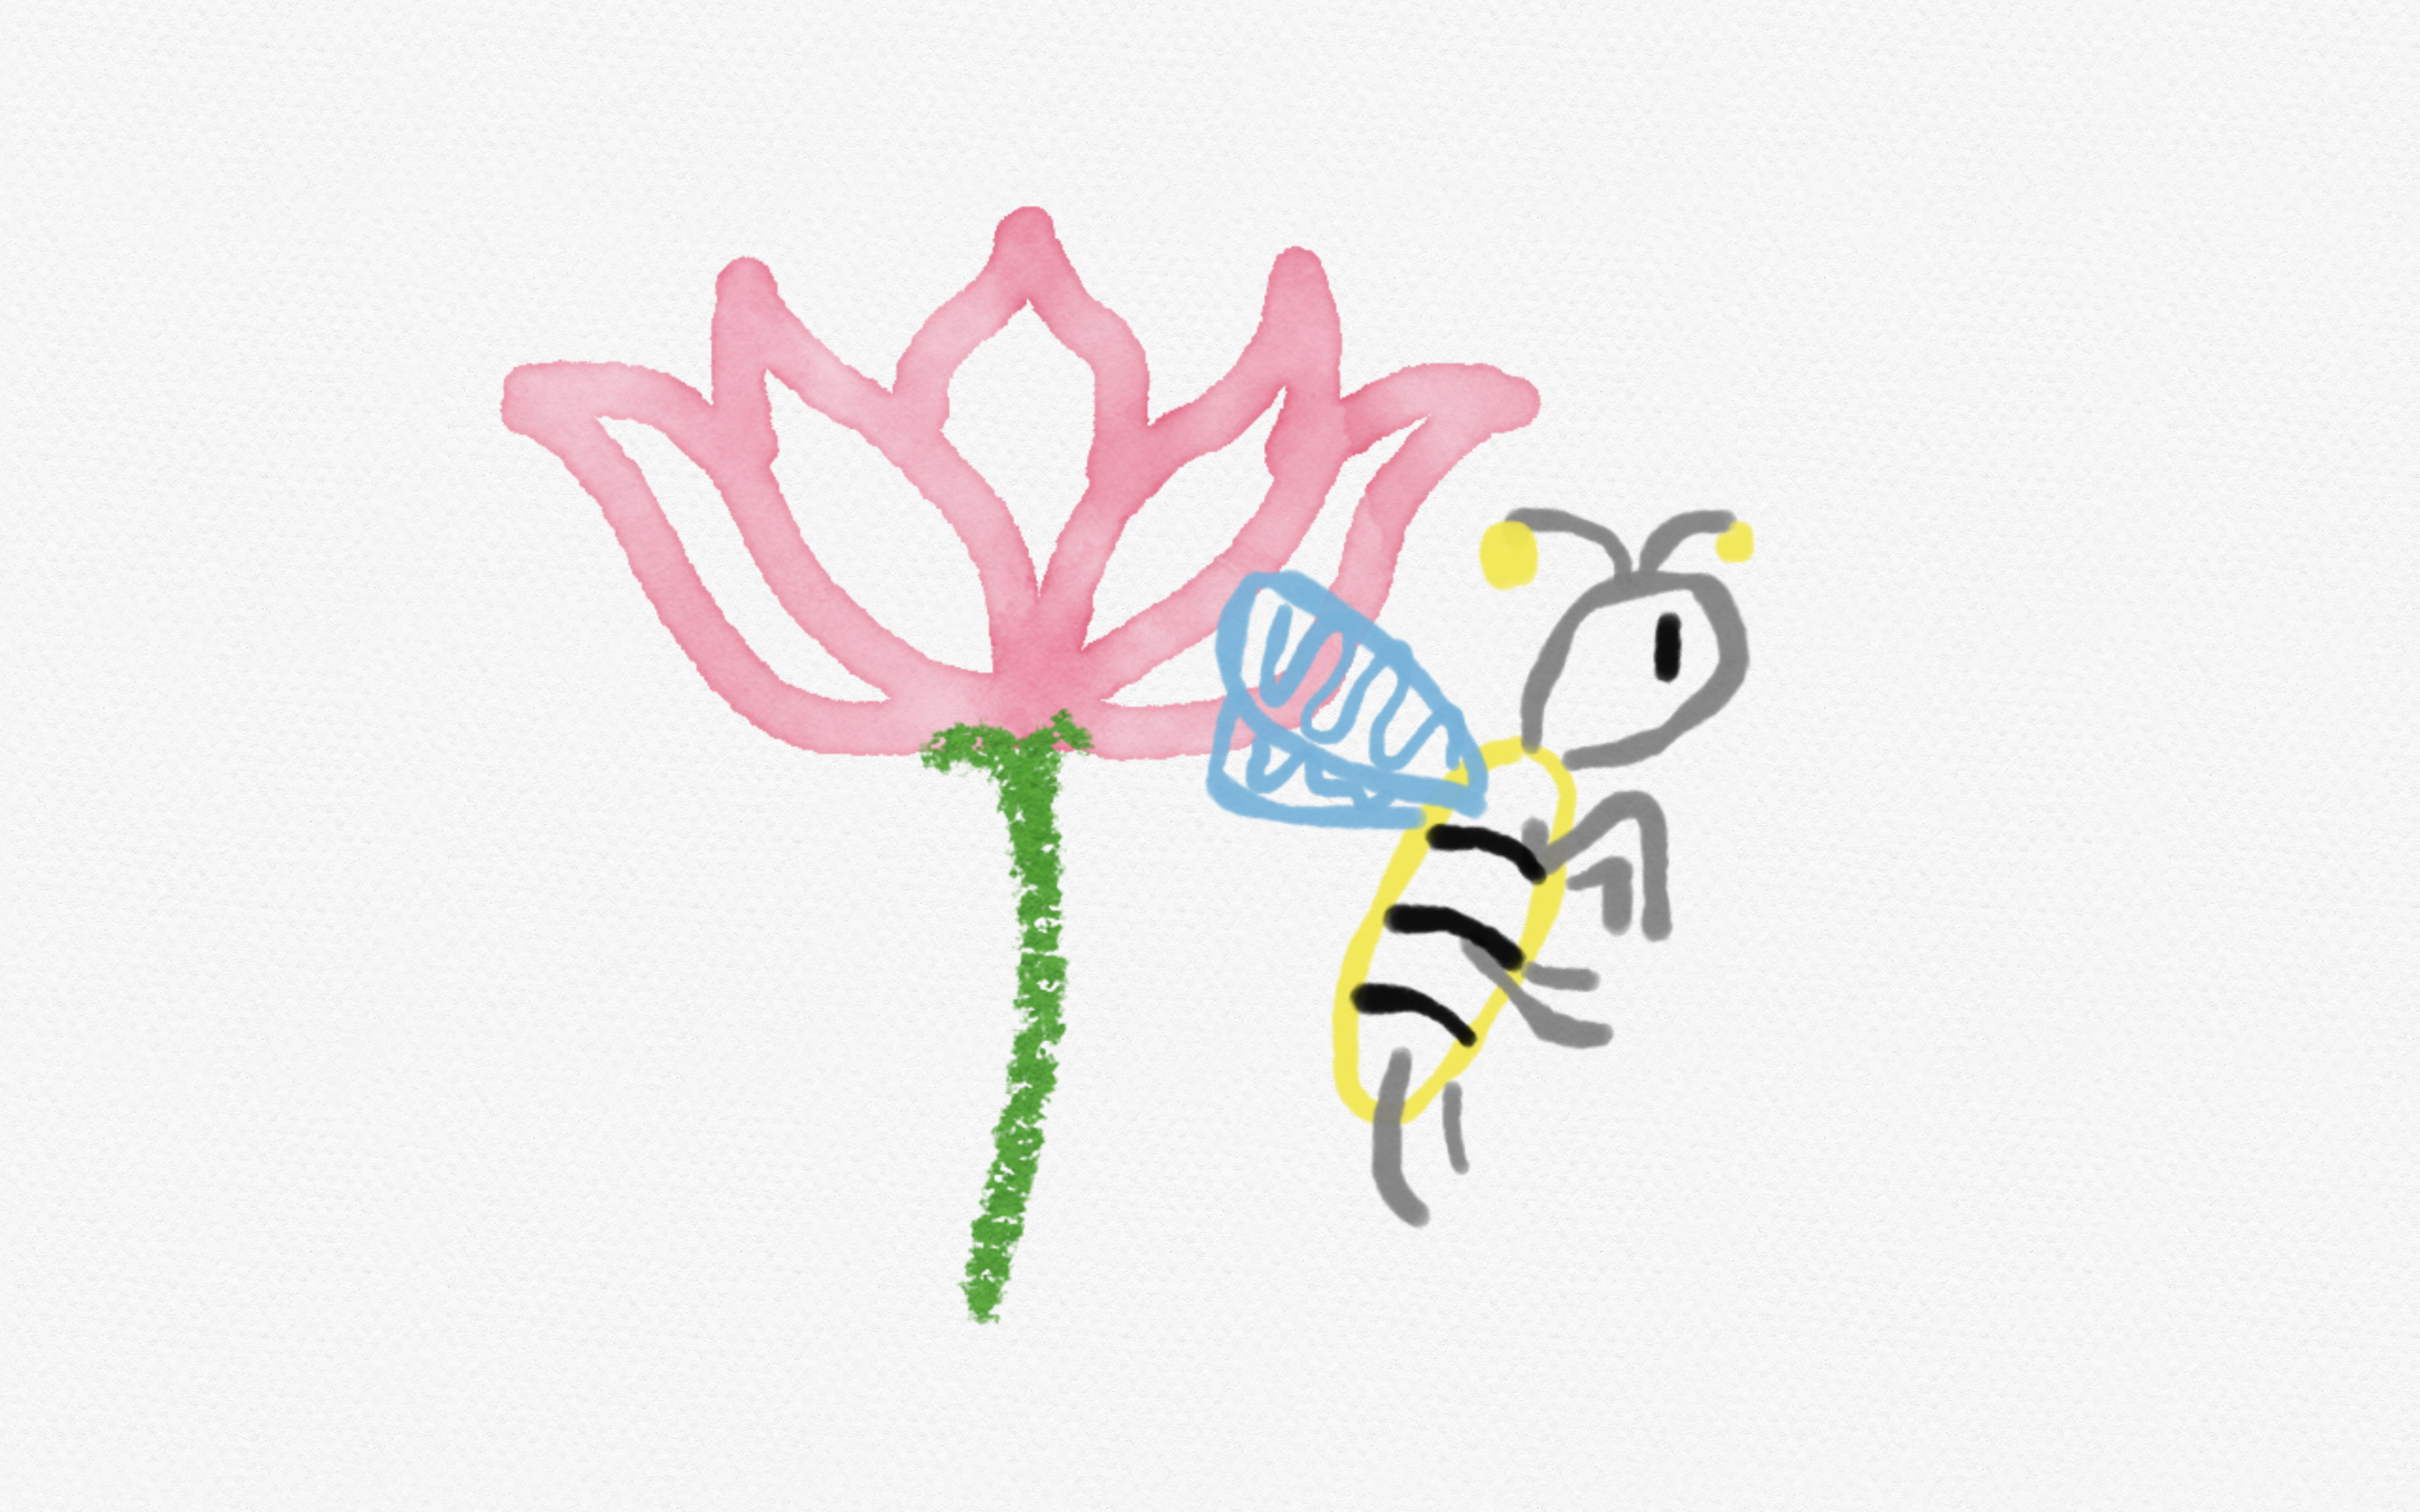
\includegraphics[width = 30em]{Logo}
\end{figure}
\newpage

\tableofcontents
\newpage

\section{Einleitung} %-------------------------------------------------------------------------------------------------
\sectionauthor{Jonas Picker}
Aufbauend auf dem Lastenheft von Christian Bachmaier und Armin Größlinger für ein Bibliothekssystem steckt unser Team, bestehend aus Sergei Pravdin, Ivan Charviakou, León Liehr, Mohamad Najjar und Jonas Picker, mit diesem Pflichtenheft den Rahmen der zu erbringenden Leistungen und verwendeten Technologien bei der Bearbeitung des Auftrags ab. Bei dem zu erstellenden System handelt es sich um eine vereinfachte Form eines Bibliotheksverwaltungssystems mit dem der Anwender das mediale Bibliotheksinventar zentral durchsuchen, kategorisieren und die Nutzung verwalten kann. Das fertige Produkt wird über einen Webbrowser bedient und bietet zahlreiche Anpassungsmöglichkeiten. Das restliche Dokument beinhaltet die genauen Spezifikationen der zu implementierenden Funktionalitäten.

\section{Zielbestimmung} %-------------------------------------------------------------------------------------------------
\sectionauthor{Jonas Picker}
\subsection{Musskriterien}
Bei der Produktinstallation auf dem Server konfiguriert der Betreiber den Webspace, spezifiziert den anzusteuernden E-Mail-Server und die zur Speicherung verwendete Datenbank. Im laufenden System zählt der Betreiber zu den Administratoren. Technische Maßnahmen sorgen dafür, dass jegliche sensible Information sicher übertragen sowie gespeichert wird und kein unbefugter Zugriff auf zugangsbeschränkte Bereiche der Anwendung durch Dritte erfolgt. Eine unterstützende Bedienungsanleitung steht für jeden nicht offensichtlichen Aspekt der Anwendung online zur Verfügung.
\begin{flushleft}
\textbf{Administratoren:} Der Betreiber ist zunächst der einzige Administrator. Administratoren können authentifizierte Nutzer in den Administratorstatus erheben sowie andere Administratoren degradieren. Administratoren sind für die Anwendungskonfiguration zuständig, welche das Setzen der institutionsspezifischen Eigenschaften (Logos, Namen, Impressum, Datenschutzerklärung etc.) sowie Variationen des Look \& Feels beinhalten. Außerdem bestimmen sie Registrierungsbedingungen und Zugangsberechtigungen für anonyme Nutzer. Ein Administrator kann die Menge der Attribute, welche alle Medien aufweisen, global bestimmen. Auch kann er die Attributwerte der einzelnen Medieninstanzen editieren, sowie Medieninstanzen erstellen, löschen und sie in hierarchische Kategorien (bis Tiefe 2) einteilen. Verwaltungs- und Übersichtsfunktionen zur Ausleihe und Rückgabe von Medien und den damit verbundenen Fristen werden außerdem bereitgestellt. Unter anderem Listenansichten der Nutzer mit überzogenen Fristen/Exemplaren sowie der zur Abholung markierten Medienexemplare. Administratoren können andere Nutzerkonten editieren und löschen, hierfür steht eine Suchfunktion bereit. Die Funktionen der authentifizierten Benutzer (und Bibliotheksmitarbeiter) stehen auch den Administratoren zur Verfügung.
\end{flushleft}
\begin{flushleft}
\textbf{Authentifizierte Nutzer:} Nach einer Validierung der E-Mail-Adresse ist ein Nutzer im System registriert und kann sich jederzeit mit seinen Accountdaten anmelden, danach kann er diese verändern und er kann sich verfügbare Exemplare von Medien zur Abholung markieren, hierzu stehen ihm die im nächsten Paragraph beschriebenen Such- und Browsingfunktionen zur Verfügung. Wird das Exemplar innerhalb einer gesetzten Frist abgeholt, gilt es als ausgeliehen und der authentifizierte Nutzer wird per E-Mail automatisch über den Ablauf der Rückgabefrist informiert. Ein angemeldeter Benutzer kann seinen Account selbstständig löschen (außer er ist der letzte Administrator oder hat noch Ausleihen zurückzugeben) und sich jederzeit abmelden.
\end{flushleft}
\begin{flushleft}
\textbf{Anonyme Nutzer:} In der Standartkonfiguration erlaubt das System Besuchern des Webspaces, neben der Registrierungsmöglichkeit, den Zugriff auf eine Such- und Browsingfunktion sowie das Herunterladen/Lesen öffentlich zugänglicher Medien. Diese Berechtigungen können von Administratoren auf die Registrierungsmöglichkeit reduziert werden. Die Suchfunktion beinhaltet die Möglichkeit sowohl nach Medien als auch nach deren Attributwerten zu suchen, sowie nach Kategorien zu filtern. Eine Detailansicht zu gefundenen Medien steht ebenfalls zur Verfügung. Um sich einen Überblick über die angebotenen Medien zu verschaffen, lässt sich die Kategoriehierarchie in Baumform zusammen mit allen einer ausgewählten Kategorie angehörenden Medien in Listenform anzeigen.
\end{flushleft}
\subsection{Wunschkriterien}
\begin{flushleft}
\textbf{Administratoren:} Bei der Zuweisung der Kategorien für Medien ist die Hierarchietiefe unbeschränkt. Zusätzlich besitzen Administratoren die Möglichkeit, einzelnen registrierten Nutzer ohne Administratorberechtigungen die Ausleihberechtigung zu entziehen bzw. zu verleihen. Hierzu gibt es eine gesammelte Ansicht der noch nicht zur Ausleihe freigeschalteten  Accounts.
\end{flushleft}
\begin{flushleft}
\textbf{Bibliotheksmitarbeiter:} Diese Nutzerrolle kann Ausleihen (direkt am Schalter und online angekündigte) abarbeiten. Um eine Abarbeitung der zur Abholung markierten Medien zu Erleichtern steht eine Listenansicht zur Verfügung. Außerdem können Mitarbeiter zurückgegebene Ausleihen wieder als verfügbar markieren. Zusätzlich ist es ihnen möglich, Attributwerte für Medien und Exemplare zu bearbeiten und neue Medien/Exemplare sowie neue Kategorien zu erstellen/löschen.
\end{flushleft}
\subsection{Abgrenzungskriterien}
Der Hauptfokus des Produkts liegt auf der Organisation und Verwaltung von Medien und Nutzern der Bibliothek, Funktionalitäten zum Erwerben und Verwalten von Lizenzen und/oder neuen Medien stehen nicht zur Verfügung. Die Abwicklung oder Verfolgung der Kundenzahlungen für Mitgliedsbeiträge, Medienerwerb o.ä. ist ebenfalls nicht im System integriert. Es besteht keine Möglichkeit, andere Bibliotheksmanagementsysteme oder Literaturenzyklopädien mit dieser Software zu verknüpfen. Das System ist für die klassische Benutzung über einen mit Tastatur, Mauszeiger und Bildschirm ausgestatteten PC/Laptop gedacht, mobile Geräte oder barrierefreie Benutzung werden begrenzt bis gar nicht unterstützt. Die Anwendung richtet sich an eine deutsche Zielgruppe und wird in der deutschen Sprache ausgeliefert. Obwohl all diese Kriterien initial nicht enthalten sind, erlaubt das modulare Entwicklungsprinzip eine Erweiterbarkeit der Anwendung um Zusatzfunktionen.

\section{Produkteinsatz} %-------------------------------------------------------------------------------------------------
\sectionauthor{Sergei Pravdin}
\subsection{Anwendungsbereich}
Das Bibliothekssystem kann in allen Bibliotheken, unabhängig von Größe, Sammelschwerpunkt, Trägerschaft und Funktion, eingesetzt werden, um Medien zu verwalten und ihren Nutzern entsprechend Zugang zu vermitteln.
\subsection{Zielgruppen}
Das System setzt keine fachspezifischen Kenntnisse voraus und richtet sich an Personen, die sich für Medien im Allgemeinen interessieren. Die Benutzeroberfläche wird auf Deutsch erstellt, entsprechend werden Deutschkenntnisse für die Anwendung des Systems vorausgesetzt. Optional soll das System in Zukunft um mehrere Sprachversionen erweitert werden. \vspace{0.5em}

Die im Folgenden aufgeführten Voraussetzungen stehen in einer hierarchischen Beziehung zueinander. Voraussetzungen, die für eine Zielgruppe definiert werden, gelten ebenfalls für alle weiteren Zielgruppen.
\subsubsection{Anonymer Nutzer}
Ein Nutzer muss über Grundkenntnisse desjenigen Internet-Browsers verfügen, den er zur Navigation durch das System zu nutzen gedenkt. Für eine Registrierung wird eine gültige E-Mail-Adresse und Zugang zu dieser vorausgesetzt.
\subsubsection{Angemeldeter Nutzer}
Für eine Anmeldung muss ein Nutzer Kenntnisse über seine Login-Daten und sein Kennwort haben. Für die Zurücksetzung eines Kennworts wird der Zugang zur E-Mail-Adresse vorausgesetzt. Für das Ausleihen und Zurückgeben der Medien werden keine Fachkenntnisse vorausgesetzt.
\subsubsection{Bibliotheksmitarbeiter}
Das System verfügt über mindestens einen Mitarbeiter, der Medien verleiht und \linebreak diese wieder zurücknimmt. Für Mitarbeiter werden keine Fachkenntnisse vorausgesetzt. Gute Kommunikationsfähigkeiten sind zu empfehlen.
\subsubsection{Administrator}
Das System hat mindestens einen Administrator, der das System einsetzt und betreibt. Dafür werden Fachkenntnisse über Datenbanken (PostgreSQL), Webservers (Tomcat) und \linebreak IT-Sicherheitsmaßnahmen vorausgesetzt.
\subsection{Betriebsbedingungen}
Das System wird von einem Administrator eingesetzt und eingestellt. Das System ist - mit Ausnahme von Updates des Betriebssystems - ständig verfügbar. Die Verfügbarkeit wird durch einen Webserver sowie einer Netz- und Datenbankverbindung sichergestellt. Diese sind durch einen Administrator bereitzustellen. Darüber hinaus muss der physische Zugriffsschutz für Server und kontinuierliche Aufsicht über das System durch einen Administrator sichergestellt werden. Tägliche Backups der Datenbank und des Dateisystems durch einen Administrator sind empfehlenswert. Optional kann das System in Zukunft so erweitert werden, dass Meldungen über geplante Wartungen und Updates im System angezeigt werden. Bei technischen Fehlern und Bugs sollen sich Nutzer an einen Administrator wenden.

\section{Produktumgebung} %-------------------------------------------------------------------------------------------------
\sectionauthor{Jonas Picker}
\subsection{Software}
Im folgenden Abschnitt werden Softwareabhängigkeiten und Kompatibilitäten des Produkts beschrieben.
\begin{itemize}
\item \underline{\textbf{Clientsoftware}}: \linebreak
Die Applikation wird über einen Webbrowser benutzt, dieser sollte die Darstellung in den Auszeichnungssprachen HTML, Version 5 und CSS, Level 3 unterstützen, sowie die Kommunikation mit dem HTTP/1.1-Protokoll. Die Unterstützung von JavaScript (ECMAScript 2020) im Browser ist ebenfalls vorausgesetzt. Explizit getestet werden die aktuellen Versionen der weit verbreiteten Browser: Google Chrome, Version: 88.0; Mozilla Firefox, Version: 85.0 und Apple Safari, Version: 14.0.3. Da HTML 5 (und CSS) zusammen mit JavaScript jedoch seit langem als Web-Standart gilt, ist Abwärtskompatibilität bei den meisten Browsern sehr wahrscheinlich.
\item \underline{\textbf{Serversoftware}}: \linebreak
Auf dem Server muss die Laufzeitumgebung 'Java Virtual Maschine' verfügbar sein, hierzu muss das 'Development Kit' OpenJDK 15.0.2 installiert und beim ebenfalls benötigten Java Enterprise Applikationsserver Apache Tomcat, Version 10.0.x registriert werden. Außerdem muss ein E-Mail-Server bereit stehen, der das SMTP-Protokoll unterstützt. Die verwendete Datenbank muss das objektrelationale Datenbankmanagementsystem PostgreSQL, Version 12 benutzen. Die Installation der JVM/Tomcat, das Aufspielen der Anwendung und des Zertifikats (siehe Orgware) sowie die Registrierung der Datenbank und des E-Mail-Servers werden in einem Installationsdokument beschrieben.
\end{itemize}
\subsection{Hardware}
Hier werden die geschätzen Rahmenbedingungen der Hardware für einen reibungslosen Betrieb in 'normaler' Belastung aufgelistet. Sollten die Rahmenbedingungen unterschritten werden, ist ein Betrieb meistens immer noch möglich, jedoch nicht garantiert.
\begin{itemize}
\item \underline{\textbf{Clienthardware}}: \linebreak
Die Bedienung der Anwendung über die oben beschriebenen Browsertypen setzt voraus, dass Clientrechner die jeweiligen Hardwareanforderungen für deren Betrieb erfüllen.
\item \underline{\textbf{Serverhardware}}: \linebreak
Die Mindestanforderungen zum Betreiben einer Datenbank unter PostgreSQL bzw. eines Applikationsservers unter Tomcat reichen für einen sinnvollen Betrieb der Anwendung unter Last nicht aus, die der Anwendung zur Verfügung stehenden Ressourcen sollten mit der Nutzerzahl in Relation stehen. Zur Speicherung der Nutzerprofile/Medien muss je nach Umfang ausreichend Datenbankspeicherplatz zur Verfügung stehen, für den anfänglichen Betrieb mindestens 1TB. Mehr Arbeitsspeicher, sowie höhere Bandbreite der Datenbank- und Internetanbindung ermöglicht dem Server ein effizienteres Bedienen vieler gleichzeitiger Anfragen. Die Architektur des Systems erlaubt es der Anwendung mit den zur Verfügung stehenden Ressourcen zu skalieren. Als Referenzplattform zum Betreiben der Anwendung dient der unten beschriebene Rechner 'schratz' für Datenbank und Server gleichermaßen.
\item \underline{\textbf{Referenzrechner}}:
\begin{flushleft}
CIP-Pool Computer 'schratz', Uni Passau, Betriebssystem: GNU/Linux Debian, Version: 4.19.132-1, 15.6GB RAM, Intel Core i7-4790 3.60GHz CPU, Intel I217-LM Ethernet Controller. \linebreak
Spezifikation der Datenbank bezieht sich auf die Referenzhardware von 'schratz'. Die Übertragungsrate zwischen Server und Datenbank beträgt ca. 1 GBit/s. Die Datenbank unterstützt das Verschlüsselungsprotokoll TLS mit einem Zertifikat. \linebreak
\end{flushleft}
\end{itemize}

\subsection{Orgware und Schnittstellen}
\begin{itemize}
\item \underline{\textbf{Client}}: \linebreak
Die notwendigen Mensch-Maschine Schnittstellen zum Benutzen der Anwendung über einen Browser sind: Bildschirm, Tastatur. Die Benutzung einer Maus oder vergleichbare Cursorsteuerung wird dringend empfohlen. Die Verifizierung eines neuen Benutzers bei der Registrierung im System wird über eine gültige E-Mail-Adresse abgewickelt, folglich muss der Nutzer Zugriff auf ein E-Mail-Konto besitzen. Der Browser des Klienten muss beim Benutzen über eine konstante Anbindung an das Internet (mind. 5 MBit/s) verfügen, eine außergewöhnlich hohe Bandbreite ist nicht erforderlich.
\item \underline{\textbf{Server}}: \linebreak
Zur initialen Installation der Anwendung und ihrer Softwareabhängigkeiten sind die selben Mensch-Maschine Schnittstellen wie beim Client notwendig. Da Administratorkonten eine E-Mail-Adresse benötigen, ist bei der Installation der Zugang zu einem E-Mail-Konto erforderlich. Auch benötigt der Server eine konstante Anbindung an das (Intra- und) Internet, um Klientenanfragen beantworten, den E-Mail-Server kontaktieren und Datenbankanfragen absetzen zu können. Die benötigte Bandbreite ist stark abhängig von der zu erwartenden Zahl der gleichzeitigen Zugriffe, für einen Minimalbetrieb mind. 25MBit/s. Um den Webspace über das Internet aufrufen zu können, muss die Domain einen Eintrag im DNS mit der festen IP des Servers besitzen. Die Datenbank kann sich auf dem gleichen Gerät wie der Server, seperat davon im Netzwerk oder geographisch getrennt 'im Internet'  befinden. Sie muss jedoch vom Server aus über einen Hostnamen ansteuerbar sein, je nach Realisierung ist dazu ein VPN-Tunnel notwendig. Um sichere Datenübertragungen mit dem TLS-Protokoll zu ermöglichen, benötigt der Tomcat-Server ein SSL-Zertifikat. Wenn sich der Server mit der Datenbank über das Internet (via SSL-VPN) verbinden soll, muss auch die Datenbank mit einem SSL-Zertifikat ausgestattet sein und die Verbindung zwischen ihr und dem Server sollte eine Bandbreite von ca. 1GBit/s aufweisen.
\end{itemize}

\section{Produktfunktionen} %-------------------------------------------------------------------------------------------------
\sectionauthor{Ivan Charviakou}

In der folgenden Aufführung unterscheidet man zwischen Administratoren, Bibliotheksmitarbeitern, registrierten Nutzern, angemeldeten Nutzern, und anonymen Nutzern.
Hierbei sind alle angemeldeten Nutzer zwangsweise auch registrierte Nutzer. Trotzdem kann ein registrierter Nutzer vor einer Authentifikation anonymer Nutzer sein.
Ferner ist die Unterscheidung zwischen einem Administrator und Bibliotheksmitarbeiter nur dann zu treffen, wenn die Rolle des Bibliotheksmitarbeiter optional umgesetzt wird.
Ansonsten sind alle Funktionen, die in dieser Aufführung nur einem Bibliotheksmitarbeiter zugeordnet sind, dem Administrator zuzuordnen. \vspace{0.5em}

Die oben genannten Rollen stehen außerdem in einer hierarchischen Beziehung zueinander.
Beispielsweise besitzt ein angemeldeter Nutzer neben den für ihn aufgelisteten Funktionalitäten auch noch alle Funktionalitäten, die einem anonymen Nutzer zustehen.
Durch eine paarweise aufsteigende Verkettung, erhält man somit die folgende Liste: Anonyme Nutzer, angemeldete Nutzer, Bibliotheksmitarbeiter, und Administratoren. \vspace{0.5em}

Zudem wird im Folgenden unter 'editieren' auch das Erstellen und Löschen gemeint, wenn nicht anders spezifiziert. \vspace{0.5em}

\subsection{Anonymer Nutzer}
	\subsubsection{Nutzerverwaltung}
		\specification{F}{90}{Wenn von Administratoren freigeschaltet, ist eine Registrierung mit einem Namen, einer Adresse, und einer gültigen E-Mail Adresse möglich.
			Dabei gilt sie nur dann als abgeschlossen, wenn auf den Link zugegriffen wird, der per Email an die angegebene Email-Adresse versendet wurde.
			Ohne diesen Schritt ist das Konto vorerst zum Ausleihen gesperrt. (\hyperlink{spec:W:70}{Siehe /W70/}) }
		\specification{F}{100}{Es ist möglich, sich mit einer registrierten E-Mail Adresse und Kennwort ins System einzuloggen. Beim Erfolg handelt es sich dann um einen angemeldeten Nutzer. }
		\specification{F}{101}{Es kann mit einer gültigen E-Mail Adresse eine Passwortzurücksetzung angefordert werden.
			Dazu wird ein Link an die angegebene E-Mail Adresse versendet, wenn sie im System registriert ist. Ansonsten verhält sich die Nutzeroberfläche in beiden Fällen gleich, um die Gültigkeit der Adresse nicht preiszugeben.
			Durch Zugriff auf diesen Link kann der Nutzer die Passwortzurücksetzung für das angegebene Nutzerkonto abschließen. }
	\subsubsection{Navigation \& Suche}
		Es ist zu beachten - Funktionalitäten, die die Anzeige von Kategorien-, Medien-, oder Exemplarenbezogene Details oder Suchergebnissen beinhalten, sind bei anonymen Nutzern nur dann vorhanden,
		wenn ihnen ein Administrator Lesezugriff auf den OPAC gewährt hat. (\hyperlink{spec:F:10}{Siehe /F10/}) \par \vspace{0.5em}
		\specification{F}{160}{Es ist möglich, mit Texteingabe nach einer Medien-Kategorie zu suchen. }
		\specification{F}{170}{Es ist möglich, durch eine Baum-Darstellung aller Kategorien im System zu navigieren. Durch Auswahl einer Kategorie, ist eine Liste von allen darin enthaltenen Medien aufrufbar. }
		\specification{F}{180}{Mit Eingabe von einer Kategorie und Werten für die jeweiligen Medienattribute kann eine Suche durchgeführt werden. }
		\specification{F}{190}{Zu einem Medium ist die Liste aller Exemplaren aufrufbar. }
		\specification{F}{191}{Der ID-Hash zu einem Medium ist kopierbar. Dabei dient der ID-Hash als Identifikator für ein Medium. (\hyperlink{spec:F:380}{Siehe /F380/}) }
		\specification{F}{210}{Die Kontaktinformationen, das Impressum, und die Datenschutzerklärung sind aufrufbar. }
		\specification{W}{230}{Es kann für eine Tabelle eingestellt werden, wie viele Datensätze pro Pagination-Seite angezeigt werden. }
	\subsubsection{Ausleihe \& Rückgabe}
		\specification{F}{191}{Falls ein Exemplar im Digitalformat frei verfügbar ist, kann es heruntergeladen werden. }
\subsection{Angemeldeter Nutzer}
	\subsubsection{Nutzerverwaltung}
		\specification{F}{110}{Nach einer erfolgreicher Anmeldung, ist es möglich, sich auszuloggen. Es handelt sich dann um einen anonymen Nutzer. }
		\specification{F}{120}{Das eigene Profil kann editiert werden. Dabei ist es nicht möglich, das Konto zu löschen, wenn die Rückgabe eines Exemplars erwartet wird.
			Die Verifikation einer neuen E-Mail Adresse erfolgt analog zu der Registrierung. (\hyperlink{spec:F:90}{Siehe /F90/}) }
	\subsubsection{Navigation \& Suche}
		\specification{F}{500}{Es kann eine Liste von ausgeliehenen und zur Abholung markierten Exemplaren aufgerufen werden. Die Rückgabefrist bzw. die Abholungsfrist wird jeweils mit angegeben. }
	\subsubsection{Ausleihe \& Rückgabe}
		\specification{F}{330}{Ein Exemplar kann zur Abholung markiert werden. (\hyperlink{spec:F:250}{Siehe /F250/}) }
\subsection{Bibliotheksmitarbeiter}
	\subsubsection{Ausleihe \& Rückgabe}
		\specification{F}{300}{Eine Liste von Exemplaren und Nutzer-E-Mails, für die der angegebene Nutzer das gegebene Exemplar zur Abholung markiert hat, ist abrufbar. }
		\specification{F}{310}{Ein Exemplar, das zur Abholung markiert ist, kann ausgeliehen werden. Ab diesem Zeitpunkt verläuft die Ausleihdauer.
			Innerhalb dieser Ausleihperiode ist das Exemplar nicht mehr zur Abholung markiert und steht anderen Nutzern nicht mehr zu Verfügung. }
		\specification{F}{320}{Ein Exemplar kann zurückgegeben werden, wodurch das Exemplar anderen Nutzern wieder zu Verfügung steht. }
		\specification{F}{321}{Ein Exemplar kann direkt ausgeliehen werden, ohne vorher vom Ausleihenden zur Abholung markiert gewesen zu sein. }
		\specification{F}{322}{Eine Abholungsmarkierung kann storniert werden. Darüber werden die betroffenen Nutzer per E-Mail benachrichtigt. }
	\subsubsection{Katalogführung}
		\specification{F}{360}{Es kann eine Kategorie editiert werden. Dabei kann sie einer anderen Kategorie als Subkategorie gehören. Dies ist mit einer Tiefe von bis zu zwei Kategorien möglich.
			Vor dem Löschen einer Oberkategorie wird auf Abhängigkeiten hingewiesen und eine Bestätigung gefordert.
			Es werden durch Löschen nur abhängige Kategorien entfernt und insbesondere keine darin enthaltene Medien. }
		\specification{F}{400}{Es kann ein Medium editiert werden. Bei der Erstellung müssen die entsprechenden Attribute gesetzt werden.
			Ein Medienverweis (\hyperlink{spec:F:380}{Siehe /F380/}) ist als ID-Hash (\hyperlink{spec:F:191}{Siehe /F191/}) einzugeben.
			Vor dem Löschen eines Mediums wird auf aktuelle Ausleihvorgänge geprüft. Falls ein zugehöriges Exemplar zu der Zeit ausgeliehen ist, wird eine Bestätigung gefordert.
			Anschließend werden alle enthaltene Exemplare mit gelöscht. }
		\specification{F}{420}{Es kann zu einem Medium ein Exemplar editiert werden. Vor dem Löschen eines Exemplar wird auf aktuelle Ausleihvorgänge geprüft.
			Falls das Exemplar zu der Zeit ausgeliehen ist, wird eine Bestätigung gefordert. Anschließend wird das Exemplar gelöscht. }
		\specification{W}{440}{Eine Kategorieverkettung von unbegrenzter Länge ist möglich. }
\subsection{Administrator}
	\subsubsection{Nutzerverwaltung}
		\specification{F}{10}{Es ist einstellbar, ob anonyme Nutzer Lesezugriff auf den OPAC haben. }
		\specification{F}{20}{Es ist einstellbar, ob neue Registrierungen im System erlaubt sind. Falls sie erlaubt sind, kann ein Regex-Ausdruck angegeben werden, der bei der Registrierung die eingegebenen E-Mail Adressen überprüft. }
		\specification{F}{30}{Ein Nutzerprofil kann editiert werden. Es lassen sich dadurch alle Nutzerdaten und die Rolle aller Nutzer verändern.
			Ausgenommen davon ist die eigene Rolle und jegliche Änderung, die dazu führt, dass es keine Administratoren mehr im System vorhanden sind.
			Beim Löschen eines Nutzers wird zuerst überprüft, ob von ihm die Rückgabe eines Exemplars erwartet wird.
			In diesem Fall wird zuerst eine Bestätigung gefordert. Anschließend werde sämtliche ausgeliehene Exemplare und leer-gewordene Medien mit gelöscht. }
		\specification{F}{60}{Es kann mit Angabe von Nutzerattributen nach Nutzern gesucht werden. Es können auch alle Nutzer im System angezeigt werden. }
		\specification{W}{70}{Nicht-administrative Benutzerkonten können von weiterer Ausleihe gesperrt und entsperrt werden. Dabei existieren zwei arten von Sperren, die für eine Ausleihe durch den Nutzer beide nicht gelten müssen.
			Eine Sperre ist frei setzbar, aber nur durch einen Administrator. Die andere Sperre kann durch einen Administrator zwar gesetzt, aber nicht aufgehoben werden.
			Dies passiert nur nämlich dann, wenn der Nutzer seine E-Mail Adresse neu verifiziert. (\hyperlink{spec:F:120}{Siehe /F120/}) }
		\specification{W}{80}{Die Liste von gesperrten Nutzerkonten ist aufrufbar. }
	\subsubsection{Ausleihe \& Rückgabe}
		\specification{F}{240}{Der Zeitabstand zwischen dem automatischen Versenden einer Email-Mahnung und der Rückgabefrist für einen beliebigen Exemplar ist setzbar.
			Dieser Wert gilt dann global für alle neue Ausleihvorgänge. Falls für einen Vorgang die Zeit bis zur Rückgabefrist kürzer ist als der gegebene Wert, wird keine Email-Mahnung versendet. }
		\specification{F}{250}{Der Zeitabstand zwischen der Abholmeldung durch einen Nutzer zu einem Exemplar und der Ausleihe dieses Exemplars ist setzbar.
			In dieser Zeit ist das Exemplar zur Abholung markiert. Zu beachten ist, dass das ausgewählte Exemplar nach Überschreiten dieser Zeit wieder allen Nutzer zu Verfügung steht. }
		\specification{F}{260}{Die Rückgabefrist für ist für alle Ausleihvorgänge einzeln setzbar. Dabei darf die Frist nicht in der Vergangenheit liegen. }
		\specification{F}{270}{Die maximale Ausleihdauer ist global, für einen bestimmten Medium, oder für einen bestimmten Nutzer setzbar.
			Wenn bei einem Ausleihvorgang mehrere Werte vorhanden sind, wird zuerst der Nutzerwert, danach der Mediumwert, und als letztes der globale Wert beachtet. }
		\specification{F}{280}{Eine Liste von Einträgen aus Nutzern, Exemplaren, und Zeitdauern, bei der der Nutzer die Rückgabefrist das gegebene Medium um die gegebene Zeitdauer überschritten hat, ist abrufbar. }
	\subsubsection{Katalogführung}
		Zu allen Medien ist eine Menge an frei definierbaren Attributen vorgesehen, mit denen Nutzer von verschiedenen Rollen bei einer Suche oder Werteingabe direkt interagieren können.
		Per Default besteht der Attributsatz aus folgenden Attributen: Index (Schlüsselkomponent), Typ, Titel, Version, Autoren (mehrwertig), Erscheinungsdatum, elektronische Version (Verweis), und Herausgeber.
		Die Attribute selber verlangen keinen Typ und es muss immer mindestens einen Attribut in dem Attributsatz vorhanden sein, der als Schlüsselkomponent markiert ist.
		Es wird garantiert, dass unter allen Medien die Gesamtheit der Attributsatzwerten, bei denen der Attribut als Schlüsselkomponent markiert ist, immer eindeutig ist. Aus diesen Werten leitet sich ein ID-Hash ab. \par \vspace{0.5em}
		\specification{F}{380}{Es kann ein neuer Attribut im Attributsatz von allen Medien definiert werden. Dieser kann als mehrwertig, als Verweis auf ein anderes Medium, oder als Schlüsselkomponent markiert werden.
			Der entsprechende Attributwert für alle Medien ist zuerst leer.
			Ist dieser Attribut als Schlüsselkomponent markiert, so wird es bei der Berechnung eines ID-Hashes verwendet und es werden dementsprechend alle Verweise im gesamten Medienbestand auf einen leeren Wert gesetzt. }
		\specification{F}{381}{Es kann ein Attribut aus dem Attributsatz von allen Medien gelöscht werden.
			Ist dieser Attribut als Schlüsselkomponent markiert, so werden zum einen alle Verweise im gesamten Medienbestand auf einen leeren Wert gesetzt.
			Zum anderen werden alle Medien nach den restlichen Schlüsselattributen zusammengefasst. Es werden nämlich alle Duplikatinstanzen gelöscht und alle zugehörige Exemplare dem verbleibenden Mediuminstanz zugeordnet.
			Falls es in Folge einer Attributlöschung eine solche Zusammenfassung stattfindet, wird zuerst eine Bestätigung für diese Löschoperation gefordert. }
	\subsubsection{Weitere Personalisierungen}
		\specification{F}{450}{Die Name der Einrichtung ist setzbar. }
		\specification{F}{460}{Das Logo der Einrichtung kann hochgeladen werden. }
		\specification{F}{470}{Das Farbenschema, bestehend aus zwei Farben, kann eingestellt werden. }
		\specification{F}{480}{Kontaktinformationen, das Impressum, und die Datenschutzerklärung sind editierbar. }

\section{Produktdaten} %-------------------------------------------------------------------------------------------------
\sectionauthor{Mohamad Najjar}

\subsection{Benutzerdaten}
\label{D010} \paragraph{/D010/ Benutzerdaten} \mbox{} \\[0.5em]

\underline{Persönliche Daten:}\\[0.5em]
\begin{tabular}{ c c }
	Vorname & Nachname \\[0.5em]
	E-Mail-Adresse (als Username) & Passwort (gehasht) \\[0.5em]
	Adresse (Ort, PLZ, Straße, Hausnummer) & Userstatus (gesperrt, offen)
\end{tabular} \\[0.5em]

\underline{Sonstige Daten:}\\[0.5em]
\begin{tabular}{ c c }
	Rolle (Siehe Produktfunktionen) 
\end{tabular} \\[0.5em]
	
\subsection{Mediumsdaten}
\label{D020} \paragraph{/D020/ Mediumsdaten} \mbox{} \\[0.5em]

\underline{Folgende Attribute sind fest:}\\[0.5em]
\begin{tabular}{ c c }
	ID & Attributhashwert \\[0.5em]
	Kategorien & Maximalausleihdauer
\end{tabular}\\[0.5em]

\underline{Die folgende Attribute sind änderbar:}\\[0.5em]
\begin{tabular}{ c c }
	Typ (Buch, CD, etc.) & Titel \\[0.5em]
	Autoren (mehrwertig) & Version \\[0.5em]
	Erscheinungsjahr & ISBN/ISSN (Index) \\[0.5em]
	Herausgeber & Link auf elektronische Version
\end{tabular}\\[0.5em]
		
\subsection{Exemplar}
\label{D030} \paragraph{/D030/ Exemplar} 
Die Operationsfrist gibt an, wann ein Exemplar abzuholen bzw. abzugeben ist. Sie bezieht sich auf den Verfügbarkeitsstatus, der folgende Werte hat: Ausgeliehen, zur Abholung markiert, verfügbar. \\[0.5em]
\begin{tabular}{ c c }
	Verfügbarkeitsstatus & Bibliothekssignatur (ID) \\[0.5em]
	Operationsfrist & Standort \\[0.5em]
	Freitext & Duplikate
\end{tabular}\\[0.5em]

\subsection{Anwendungs- und Einrichtungsdaten}
\label{D040} \paragraph{/D040/ Anwendungs- und Einrichtungsdaten} \mbox{} \\[0.5em]
\begin{tabular}{ c c }
	Name des Betreibers & Akzeptierte E-Mail Domäne (RegEx) \\[0.5em]
	Registrierungsstatus (offen, geschlossen) & Impressum mit Kontaktdaten \\[0.5em]
	Logo & Datenschutzerklärung \\[0.5em]
	Ausleihfrist (global) & Abholungsfrist (global) \\[0.5em]
	Mahnungszeitversatz & Anonymes Lesen (Ja, Nein)  
\end{tabular}\\[0.5em]
	
\subsection{Kategorie}
\label{D050} \paragraph{/D050/ Kategorie} \mbox{} \\[0.5em]
\begin{tabular}{ c c }
	ID & Titel \\[0.5em]
	Elternkategorie & Beschreibung
\end{tabular}
	
\section{Produktleistung} %-------------------------------------------------------------------------------------------------
\sectionauthor{Mohamad Najjar}

\subsection{Benutzerfreundlichkeit}

     \paragraph{/L010/ \label{L010} Bedienbarkeit}
    Ein klares Design der Webanwendung ermöglicht eine einfache und intuitive Bedienung. Die häufig verwendeten Funktionen sind leicht zugänglich. Eine Suchfunktion ist auch  verfügbar. Damit lassen sich Dateien und Einträge leicht finden.
    
     \paragraph{/L020/ \label{L020} Zeichenkodierung} Die Texte  der Website sind UTF-8 kodiert.
     
      \paragraph{/L030/  \label{L030} Online-Hilfe} Dem Benutzer wird zu jeder Seite eine konextsensitive Online-Hilfe angeboten
      
      \paragraph{/L040/ \label{040} Installation}
      Eine schnelle und komfortable Installation für Systembetreiber ist vorgesehen, die auch eine automatische Konfiguration der Datenbank beinhaltet.
      
      \paragraph{/L050/ \label{L050} Eingabe}
      Bei einer fehlerhaften Eingabe in ein HTML-Formular wird eine kumulierte Fehlermeldung zurückgegeben. Felder, die bereits ausgefüllt wurden, müssen nicht erneut eingegeben werden.
      
      \paragraph{/L060/ \label{L060} Tabellen}
      
    Alle Tabellen sind nach ihren jeweiligen Spalten sortierbar. Tabellen,
    die eine bestimmte Anzahl von Einträgen überschreiten, werden durch Paginierung auf mehrere Seiten aufgeteilt, deren Länge einstellbar ist. Per Default beträgt die Paginierungslänge 
      
      
\subsection{Zuverlässigkeit und Sicherheit}
   \paragraph{/L070/ \label{070} Datenspeicherung}
   Alle dynamisch veränderbaren Daten werden persisten in einer PostgreSQL-Datenbank gespeichert. Die Konsistenz der Daten ist auch im Mehrbenutzerbetrieb gewährleistet. Im Fall wenn  Änderungen mehrere Datenbanktabellen betreffen, werden Transaktionen verwendet.
  
   \paragraph{/L080/ \label{080} Datenlöschen}
   
  Bestehen Abhängigkeiten ( z.B der Administrator möchte ein Medium löschen und dieses Medium hängt mit anderem Datensatz ab dann wird er  darauf hingewiesen bevor  er  löschen möchte)  zwischen den zu löschenden Daten und anderen Datensätzen, werden diese erst nach einer Warnung an den Benutzer gelöscht.
  
\subsubsection{Datenschutz}
	\paragraph{/L090/ \label{L090} 
	Personenbezogenen Daten} 
	Alle Benutzerdaten, wie z. B. Login-Daten, werden ausschließlich über eine SSL-Verbindung übertragen. Der Zugriff auf sensible Daten durch unbefugte Dritte wird so weit wie möglich verhindert.
		    
	\paragraph{/L100/ \label{L100} Transparenz}
    Technische Informationen über das System können nicht von außen eingesehen werden.
		   
   \paragraph{/L110/ \label{L110} Passwörter} Passwörter werden gehashed gespeichert.
   
    \paragraph{/L120/ \label{L120} HTML und CSS}
    Das System ist durch valides HTML und CSS aufgebaut.
    
    \paragraph{/L130/ \label{L130} Schutz gegen Manipulationen} Eine Manipulation mit den üblichen Angriffsmethoden wie SQL-Injection oder Cross-Site-Scripting ist ausgeschlossen. Darüber hinaus sind die Benutzer vor Session Hijacking geschützt.
   
    \paragraph{/L140/ \label{L140} Benutzerdaten}
   Alle Benutzerdaten sind nur für autorisierte Benutzer zugänglich.
   Ein unberechtigter Zugriff durch Dritte oder andere Benutzer ist ausgeschlossen.

   \paragraph{/L150/ \label{L150} Cookies}
   Cookies werden nciht erzwungen.
   
   \paragraph{/L160/ \label{L160} Logging}
    Das System besitzt einen Logger, welcher das Auftreten von untyptischen Verhalten in einer Logdatei festhält.

 \subsection{Skalierbarkeit und Performance}
	        \paragraph{
	        /L170/ \label{L170} Last}
	       Die Anwendung ist in der Lage sein, mindestens 20 Anfragen pro Sekunde unter realistischer Lastverteilung auf einem Referenzplattform (CIP-Pool-Rechner) zu beantworten. Bei einer Last von 20 Anfragen pro Sekunde werden 90\% der Anfragen nicht mehr als 3 Sekunden beantwortet.
	       \paragraph{
	        /L180/ \label{L180} Erweiterbarkeit} Das System ist so aufgebaut, dass eine weitere Entwicklung zu  realisieren  ist.
	
\subsection{Wunschkriterien}
	    \paragraph{/LW190/ \label{LW190} Sprache}
	    Das System ist auch in anderen Sprachen verfügbar, z. B. in Englisch.
	    
\paragraph{/LW200/ \label{LW210} Farbschema}	    	       
	       Mit der Farbwahl ist es möglich, die Darstellung der betreibenden Einrichtung durch das Erscheinungsbild der Webanwendung anzupassen.

\section{Benutzeroberfläche} %-------------------------------------------------------------------------------------------------
\sectionauthor{León Liehr}

In den Abbildungen \ref{katstoeb}, \ref{katstoebmit}, \ref{mediumsansicht}, \ref{mediumsansichtmit} und \ref{mediensuche} werden die einzelnen Unterseiten der Webapplikation skizzenhaft dargestellt.

\begin{figure}[h]
    \centering
    \includegraphics[width = 20em]{Kategorienstöberer}
    \caption{Skizzierung des Kategorienstöberers aus Sicht eines nicht angemeldeten Nutzers}
    \label{katstoeb}
\end{figure}

\begin{figure}[h]
    \centering
    \includegraphics[width = 20em]{Kategorienstöberer_Mitarbeiter}
    \caption{Skizzierung des Kategorienstöberers aus Sicht eines Bibliotheksmitarbeiters}
    \label{katstoebmit}
\end{figure}

\begin{figure}[h]
    \centering
    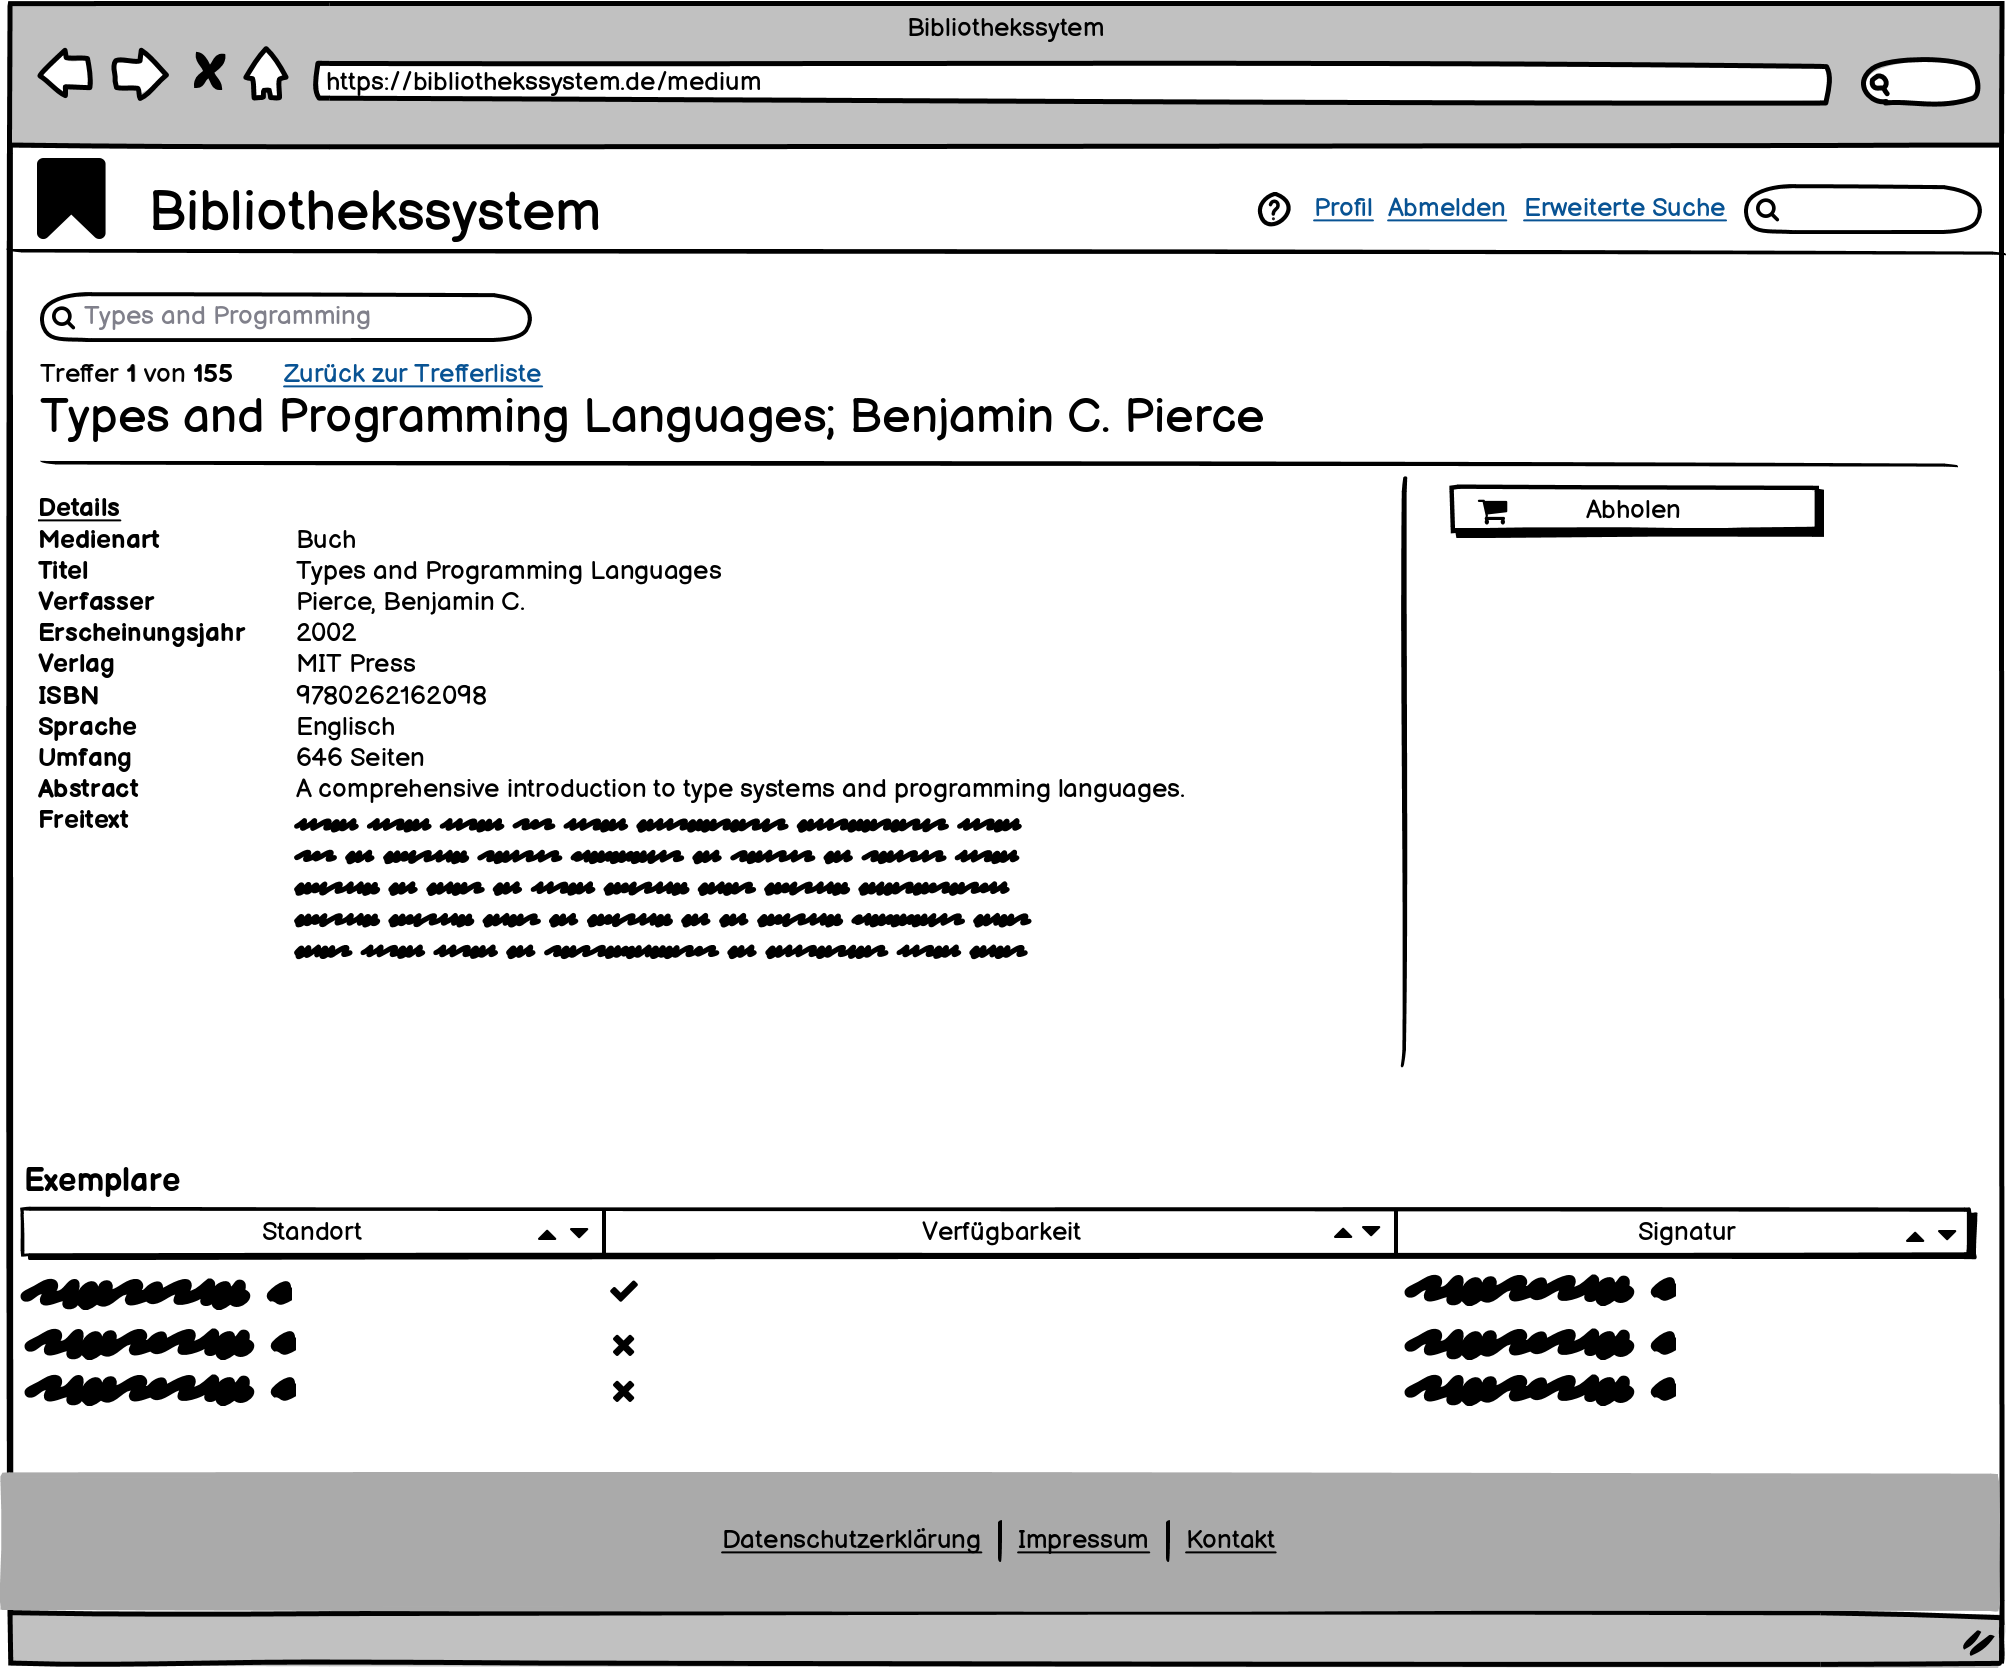
\includegraphics[width = 20em]{Mediumsansicht}
    \caption{Skizzierung der Mediumsansicht aus Sicht eines angemelden Nutzers}
    \label{mediumsansicht}
\end{figure}

\begin{figure}[h]
    \centering
    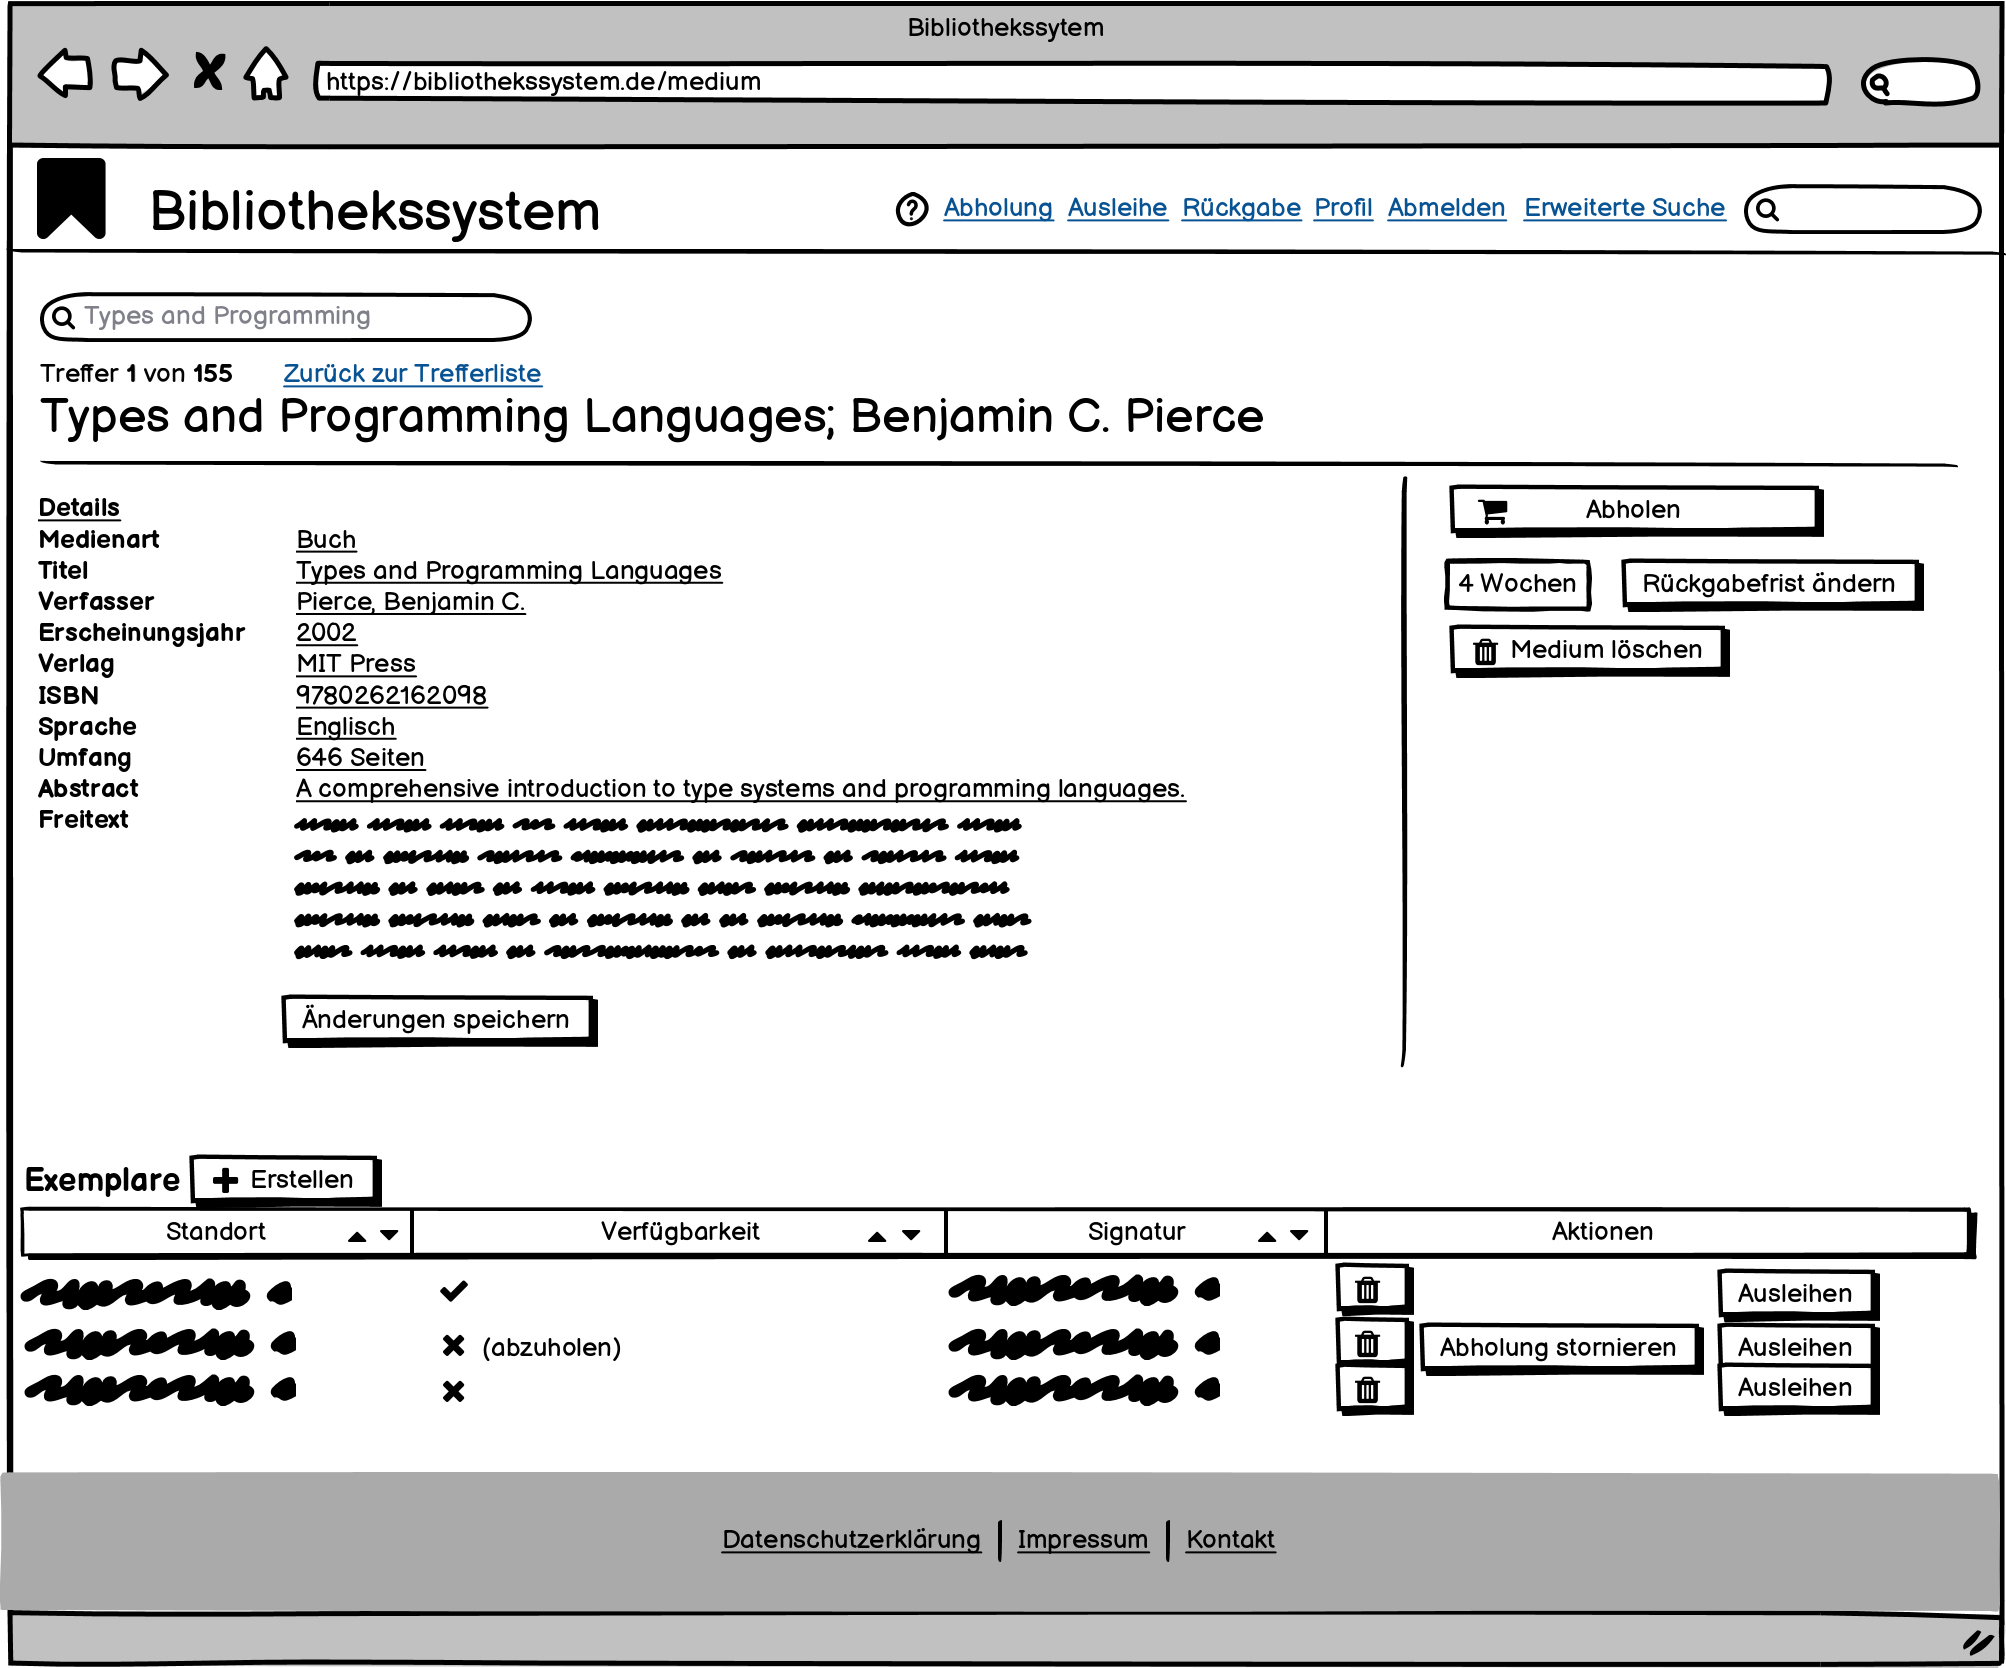
\includegraphics[width = 20em]{Mediumsansicht_Mitarbeiter}
    \caption{Skizzierung der Mediumsansicht aus Sicht eines Bibliotheksmitarbeiters}
    \label{mediumsansichtmit}
\end{figure}

\begin{figure}[h]
    \centering
    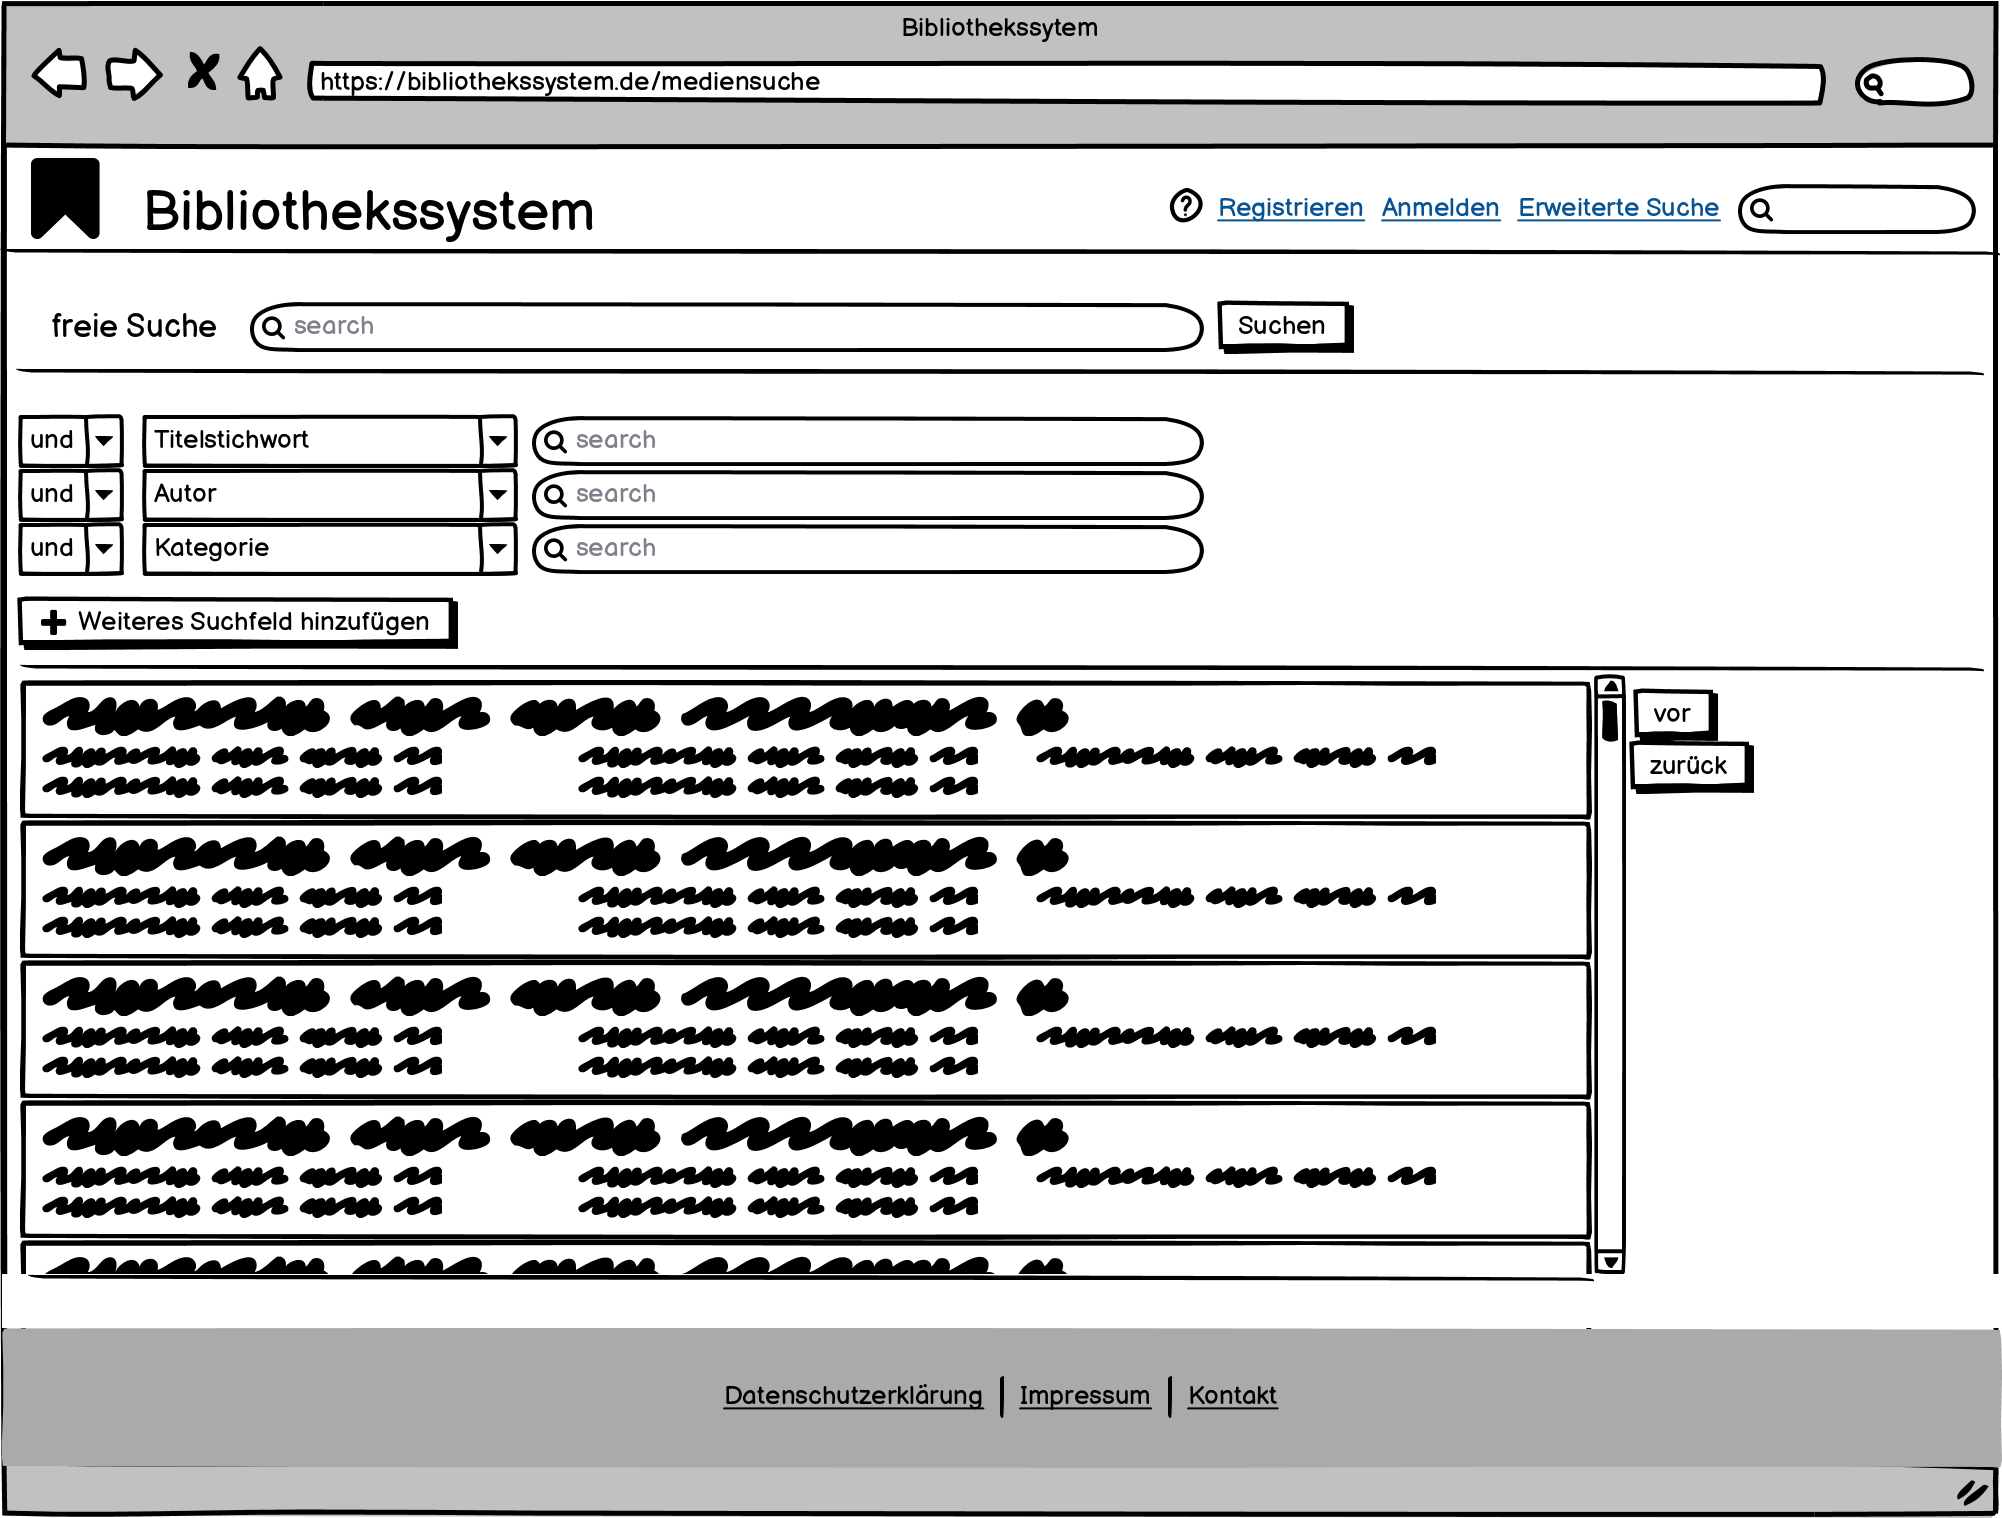
\includegraphics[width = 20em]{Mediensuche}
    \caption{Skizzierung der Mediensuche aus Sicht eines nicht angemeldeten Nutzers}
    \label{mediensuche}
\end{figure}

\newpage
\newgeometry{left=0cm,right=0cm,top=0cm,bottom=0cm}

\begin{figure}[h]
    \centering
    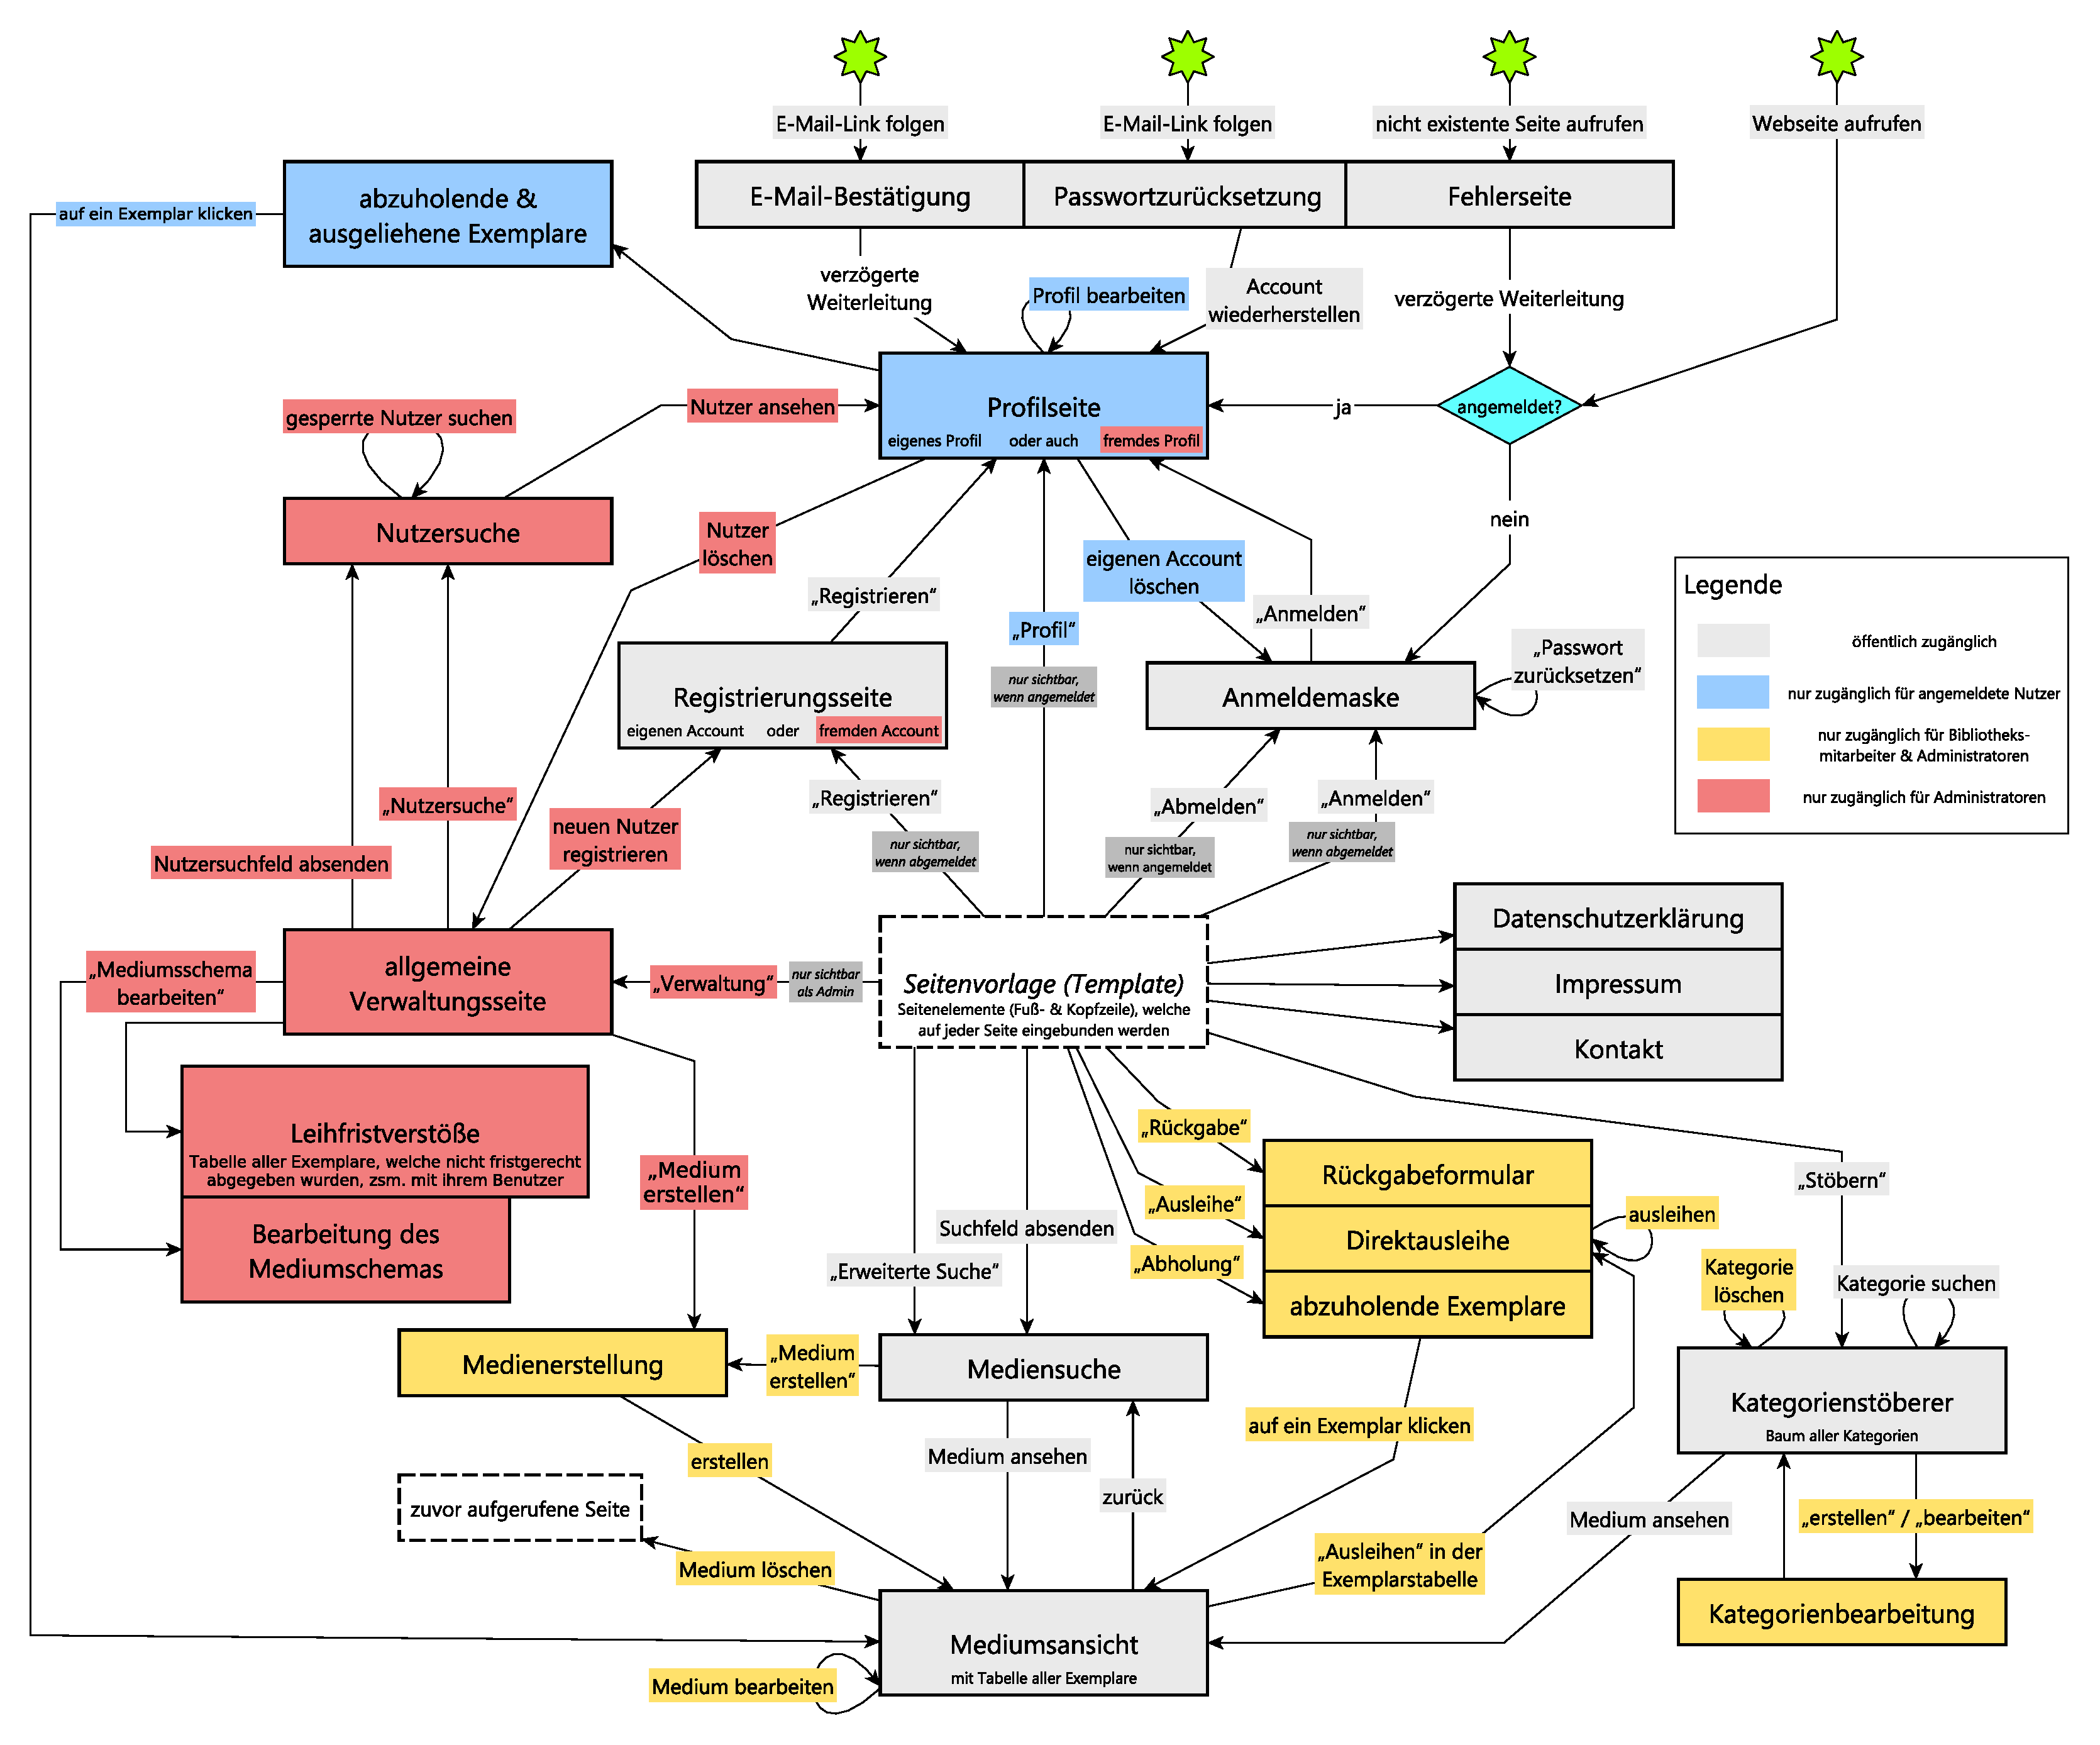
\includegraphics[angle = 270, width = 60em]{site_map}
    \caption{Die Inhaltsübersicht der Webseite (engl. \textit{site map})}
    \label{site_map}
\end{figure}

\restoregeometry
\newpage

\section{Qualitätsanforderungen} %-------------------------------------------------------------------------------------------------
\sectionauthor{Mohamad Najjar}

Die folgende Tabelle zeigt die Priorität, die jeder Qualitätsanforderung zugewiesen wird.
	
\begin{center}
\begin{tabular}{ |l||c|c|c|c| } 
 \hline
  & sehr wichtig & wichtig & weniger wichtig &\\
 \hline\hline
 Benutzerfreundlichkeit & X & & & \\
 \hline
 Funktionalität & X & & & \\ 
 \hline
 Korrektheit & X & & & \\
 \hline
 Robustheit & & X & & \\
 \hline
 Vertrauenswürdigkeit & & X & & \\
 \hline
 Effizienz & & X & & \\
 \hline
 Änderbarkeit & & X & & \\
 \hline
 Portierbarkeit & &   & X & \\

 \hline
\end{tabular}
\end{center}
\begin{itemize}
\item Da  unser System einfach und intuitiv zu bedienen sein soll und die häufigsten Funktionen sollten
 zugänglich sein, wird sehr wichtig  auf die Benutzerfreundlichkeit und Funktionalität gesetzt.
\item Aus dem Grund, dass sensible Daten zu jedem Zeitpunkt nur für Berechtigte zugänglich sind, wird auf  wichtig gesetzt.
\item Um Manipulationen mit bekannten Angriffsmethoden zu verhindern, werden bestimmte Maßnahmen getroffen.
\end{itemize}

\section{Blackbox-Tests} %-------------------------------------------------------------------------------------------------
\sectionauthor{Sergei Pravdin}
Das Bibliothekssystem ist erfolgreich eingesetzt und so eingestellt, dass eine Registrierung für alle E-Mail-Domänen möglich ist. Das System hat einen Administrator namens Max Mustermann mit der E-Mail-Adresse 'admin.sep2021.test@gmail.com', der Anschrift 'Innstraße 33, 94032 Passau, Deutschland' und dem Kennwort 'xlA24!bGhm'. Außerdem verfügt das Impressum in der Anschrift die Innstraße. \vspace{0.5em}

Die im Folgenden beschriebenen Testfälle bauen aufeinander auf. Das bedeutet, dass der Zustand des Systems für den folgenden Testfall übernommen wird.
\subsection{Testfälle}
\specification{T}{010}{Die Webseite des Systems wird aufgerufen. Der Administrator gibt die E-Mail-Adresse 'admin.sep2021.test@gmail.com' und das Kennwort 'xlA24!bGhm' in die Anmeldungsfelder 'E-Mail-Adresse' und 'Passwort' ein und klickt auf 'Anmelden'. Die Anmeldung ist erfolgreich und die Profilseite mit dem Nachnamen 'Mustermann' wird gezeigt. ­­­­­ (\hyperlink{spec:F:100}{/F100/}) }
\specification{T}{011}{Der Administrator klickt auf 'Allgemeine Verwaltungsseite' und dann auf 'Mediumsschema bearbeiten'. Er gibt '00:00:01' (1 Minute) im Feld Ausleihdauer ein und klickt auf 'Speichern'. Die Seite 'Bearbeitung des Mediumsschemas' wird erneut geladen und die Ausleihdauer '00:00:01' ist sichtbar. (\hyperlink{spec:F:240}{/F240/}) (\hyperlink{spec:F:270}{/F270/})}
\specification{T}{020}{Der Administrator klickt auf 'Verwaltung' und im Anschluss auf 'Neuen Nutzer registrieren'. Die Registrierungsseite wird geladen und der Administrator gibt im Registrierungsformular als E-Mail-Adresse, Kennwort, Vorname, Name, Straße, Hausnummer, PLZ, Stadt, Land folgende Daten an:  'mitarbeiter.sep2021test@gmail.com', 'sijAs13!!A', 'Tom', 'Mustermann', 'Instraße', '33', '94032', 'Passau', 'Deutschland'. Anschließend klickt er auf 'Bearbeiten', definiert die Rolle des Profiles als 'Mitarbeiter' und klickt auf 'Speichern'. Danach klickt er auf 'Registrieren', 'Abmelden' und gibt die E-Mail-Adresse 'mitarbeiter.sep2021test@gmail.com' sowie das Kennwort 'sijAs13!!A' in die Anmeldungsfelder 'E-Mail-Adresse' und 'Passwort' ein. Er klickt auf 'Anmelden'. Die Anmeldung ist erfolgreich und die Profilseite mit dem Nachnamen 'Mustermann' und mit dem Vornamen 'Tom' wird gezeigt. (\hyperlink{spec:F:110}{/F110/}) (\hyperlink{spec:F:30}{/F30}) }
\specification{T}{030}{Der Mitarbeiter klickt auf 'Profil bearbeiten', setzt 'Müller' als Nachname und klickt auf 'Speichern'. Die Profilseite wird wiedergeladen und der Nachname 'Müller' ist sichtbar. ­­­­­ (\hyperlink{spec:F:120}{/F120/}) }
\specification{T}{040}{Der Mitarbeiter klickt auf 'Erweiterte Suche', im nächsten Schritt auf 'Medium erstellen', gibt im Formular '17RE', 'Buch', 'Programmieren lernen', '1.0', 'Mustermann', '2020', 'Springer' als 'Index', 'Typ', 'Titel', 'Version', 'Autoren', 'Erscheinungsdatum' und 'Herausgeber' ein und klickt auf 'Erstellen'. Die Seite des Mediums wird geladen und der Index '17RE' ist sichtbar. ­­­­­ (\hyperlink{spec:F:380}{/F380/}) (\hyperlink{spec:F:400}{/F400/})}
\specification{T}{050}{Der Mitarbeiter befindet sich auf der Seite des Mediums 'Programmieren lernen' und klickt 'Medium bearbeiten'. In der Tabelle aller Exemplare gibt er die Signatur '17RE (+1)' ein und klickt im Anschluss auf 'Speichern'. Die Seite wird erneut geladen und die Signatur 17RE (+1)' ist sichtbar. ­­­­­ (\hyperlink{spec:F:420}{/F420/}) (\hyperlink{spec:F:190}{/F190/})}
\specification{T}{060}{Der Mitarbeiter klickt auf 'Stöbern', dann auf 'Kategorie erstellen' und gibt im Formular 'Informatik' und 'Alle Medien zu Informatik' als 'Name', und 'Beschreibung' ein. Anschließend klickt er auf 'Speichern'. Der Kategorienstöberer wird geladen und die Kategorie 'Informatik' ist sichtbar. ­­­­­ (\hyperlink{spec:F:360}{/F360/})}
\specification{T}{070}{Der Mitarbeiter gibt im Suchfeld 'Programmieren lernen' ein und sendet den Suchauftrag ab. Die Seite 'Mediensuche' wird geladen und das Medium mit Titel 'Programmieren lernen' ist sichtbar. Im nächsten Schritt klickt der Mitarbeiter auf dieses Medium, die Seite des Mediums wird geladen. Danach klickt der Mitarbeiter auf 'Medium bearbeiten', definiert im Attributsformular die Kategorie 'Informatik­­­­­' und klickt dann auf 'Speichern'. Er klickt nun auf 'Stöbern', der Kategorienstöberer wird geladen und das Medium ist mit dem Titel 'Programmieren lernen' unter der Kategorie 'Informatik' im Baum aller Kategorien sichtbar.  (\hyperlink{spec:F:160}{/F160/}) (\hyperlink{spec:F:170}{/F170/})}
\specification{T}{080}{Der Mitarbeiter klickt auf 'Abmelden' und im nächsten Schritt auf 'Impressum'. Die Seite mit dem Impressum wird geladen und 'Innstraße' wird in der Anschrift auf der Seite sichtbar. ­­­­­ (\hyperlink{spec:F:210}{/F210/})}
\specification{T}{090}{Der Nutzer gibt im Suchfeld 'Informatik Springer' ein und sendet die Suchanfrage ab. Die Seite zur Mediensuche wird geladen und das Medium mit dem Titel 'Programmieren lernen' ist sichtbar. ­­­­­ (\hyperlink{spec:F:180}{/F180/})}
\specification{T}{100}{Der Nutzer klickt auf 'Registrierung'. Die Registrierungsseite wird geladen und der Nutzer gibt im Registrierungsformular als E-Mail-Adresse, Kennwort, Vorname, Name, Straße, Hausnummer, PLZ, Stadt, Land folgende Daten ein: 'nutzer.sep2021test@gmail.com', 'sdfHs4!a', 'Bob', 'Mustermann', 'Innstraße', '40', '94032', 'Passau', 'Deutschland'. Danach klickt er auf 'Registrieren'. Anschließend bestätigt er seine E-Mail-Adresse durch den Verifizierungslink. Die Anmeldung ist erfolgreich und als Ergebnis wird die Profilseite mit dem Vornamen 'Bob' und der E-Mail-Adresse 'nutzer.sep2021test@gmail.com' angezeigt.  ­­­­­ (\hyperlink{spec:F:90}{/F90/})}
\specification{T}{110}{Der Nutzer klickt auf 'Abmeldung', gibt als E-Mail-Adresse \linebreak  'nutzer.sep2021test@gmail.com' ein und klickt auf 'Passwort vergessen'. Anschließend \linebreak  bestätigt er seine E-Mail-Verifizierung durch den Verifizierungslink. Die Wiederherstellungsseite wird geladen und der Nutzer gibt im Wiederherstellungsformular zwei Mal das neue Kennwort 'djnASdd1d!' ein. Anschließend klickt er auf 'Speichern'; es wird eine Profilseite als Ergebnis geladen. Auf der Seite ist der Vorname 'Bob' sichtbar.­(\hyperlink{spec:F:101}{/F101/})}
\specification{T}{120}{Der Nutzer klickt auf 'Stöbern' und auf das Medium 'Programmieren lernen'. Anschließend klickt er auf 'Buchen'. Die Mediumseite wird wiedergeladen und der Status des Exemplars 'Gebucht' ist sichtbar. ­­ (\hyperlink{spec:F:330}{/F330/})}
\specification{T}{130}{Der Nutzer klickt auf 'Abmelden' und wird auf die Anmeldungsseite weitergeleitet. Er gibt dort die E-Mail-Adresse 'mitarbeiter.sep2021test@gmail.com' und das Kennwort 'sijAs13!!A' in die Formularfelder 'E-Mail-Adresse' und 'Passwort' ein und klickt auf 'Anmelden'. Nach erfolgreicher Anmeldung navigiert er durch einen Klick auf 'Abholung' zur Listenansicht der abzuholenden Exemplare. Die Seite wird geladen und der Mitarbeiter klickt auf 'abgeholt' bei dem Listeneintrag mit der Signatur '17RE (+1)'. Die Seite wird erneut geladen und der Eintrag mit der Signatur '17RE (+1)' ist verschwunden.(\hyperlink{spec:F:300}{/F300/})\hyperlink{spec:F:310}{/F310/}) }
\specification{T}{140}{Nach einer Minute klickt der Mitarbeiter auf 'Rückgabe' und die Seite mit dem Rückgabeformular wird geladen. Der Mitarbeiter gibt die Signatur '17RE (+1)' und die E-Mail-Adresse \linebreak 'nutzer.sep2021test@gmail.com' in die entsprechenden Formularfelder ein und klickt anschließend auf \linebreak 'Bestätigen'. Eine entsprechende Meldung über die erfolgreiche Zurücknahme wird sichtbar. (\hyperlink{spec:F:300}{/F300/})\hyperlink{spec:F:320}{/F320/}) }
\specification{T}{150}{Der Mitarbeiter klickt auf 'Ausleihe' und gibt auf der Seite 'Direktausleihe' im Formular die Signatur '17RE (+1)' und die E-Mail-Adresse 'nutzer.sep2021test@gmail.com' ein und bestätigt seine Eingabe. Somit ist die direkte Ausleihe erfolgreich abgeschlossen und eine entsprechende Meldung auf der Seite sichtbar ist. (\hyperlink{spec:F:321}{/F321/})}
\specification{T}{160}{Der Mitarbeiter klickt auf 'Abmelden' und die Anmeldungsmaske wird geladen. Der Administrator gibt die E-Mail-Adresse 'admin.sep2021.test@gmail.com' und das Kennwort 'xlA24!bGhm' in die Anmeldungsfelder 'E-Mail-Adresse' und 'Passwort' ein und klickt auf 'Anmelden'. Nach erfolgreicher Anmeldung klickt er auf 'Verwaltung' und navigiert zur Listenansicht 'Leihfristverstöße'. Nach dem Laden der Seite ist das Exemplar mit der Signatur '17RE (+1)', sowie der Nutzeraccount mit der E-Mail 'nutzer.sep2021test@gmail.com' und die Zeitangabe der überzogenen Frist ist sichtbar.(\hyperlink{spec:F:280}{/F280/})}
\specification{T}{170}{Der Administrator klickt auf 'Verwaltung', navigiert von dort aus zur Nutzersuche und gibt nach laden der Seite 'Bob Mustermann' im Suchfeld ein. Anschließend sendet er die Suchanfrage an und die Seite 'Nutzersuche' wird geladen, auf der der Nutzer 'Mustermann' sichtbar ist.(\hyperlink{spec:F:60}{/F60/})}
\specification{T}{180}{Der Administrator klickt auf 'Verwaltung' und dann auf 'Bearbeiten'. Im Formular gibt er 'grün', 'gelb' und 'Testsystem' in die Felder 'Farbe 1' , 'Farbe 2' und 'Name der Einrichtung' ein. Schließlich klickt er auf 'Speichern'. Die 'Allgemeine Verwaltungsseite' wird erneuet geladen und die Farben 'grün' und 'gelb', sowie der Name 'Testsystem' sind auf der Seite sichtbar. (\hyperlink{spec:F:450}{/F450/}) (\hyperlink{spec:F:470}{/F470/})}
\specification{T}{190}{Der Administrator klickt auf 'Impressum' und dann auf 'Bearbeiten'. Im Formular gibt er 'Germany' im Feld 'Land' ein. Schließlich klickt er auf 'Speichern'. Die Seite 'Impressum' wird erneuet geladen und das Land 'Germany' auf der Seite sichtbar.(\hyperlink{spec:F:480}{/F480/})}

\section{Entwicklungsumgebung} %-------------------------------------------------------------------------------------------------
\sectionauthor{Jonas Picker}
Die Entwicklung finden auf verschiedenen Privatrechnern der Teammitglieder statt, deren Bauteile und Betriebssysteme und verwendete Software im Folgenden kurz umrissen werden. Keiner der Rechner weißt sonstige Besonderheiten auf.
\subsection{Software}
Siehe Tabelle 1.
\begin{center}
\begin{table}
\caption{\textsc{Softwareauflistung}}
\begin{adjustwidth}{-1.5cm}{-1cm}
\begin{tabular} { c c }
\underline{\textbf{Dokumentenbearbeitung}} & \underline{\textbf{Webbrowser}} \\
-LaTeX-Editor TeXworks, Version: 0.6.6 &-Google Chrome, Version: 88.0 \\
-Overleaf Online Latex Editor &-Mozilla Firefox, Version: 85.0 \\
-LaTeX Distribution MacTeX-2021 &-Apple Safari, Version: 14.0.3 \\
-LaTeX-Editor TeXShop, Version: 4.62 (siehe IDEs) & \underline{\textbf{Integrierte Entwicklungsumgebungen}} \\
-LaTeX Distribution TeX Live, Version: 2021 &-Visual Studio Code, Version: 1.55.2 \\
-Dokumentenbetrachter Evince, Version: 3.38.1 &-Eclipse IDE for JavaEE, Version: 2020-12(4.18.0) \\
-LaTeX-Bearbeitung mit IntelliJ (siehe IDEs) &-IntelliJ IDEA 2021.1 Ultimate Edition \\
-LaTeX-Editor TeXstudio, Version: 3.1.1 & \underline{\textbf{Objektorientierte Modellierung}}\\
-Vim, Version: 8.2 &-IBM Rational Software Architect Designer 9.7 \\
-LaTeX Distribution MiKTeX, Version: 21.2 & \underline{\textbf{Programmiersprachen, Entwicklungs- \& Testframeworks}}\\
\underline{\textbf{Versionsmanagement}} &-Java OpenJDK 15.0.2 GA-Release von https://jdk.java.net/15/ \\
-git, Version 2.31.1 &-Jakarta EE 9\\
\underline{\textbf{Projektmanagement}} &-Jakarta Server Faces 3.0 Mojarra Implementation\\
-Microsoft Project, Version: 2019 &-CDI 3.0 with Red Hat Weld, Version: 4.0.1.Final\\
\underline{\textbf{Betriebssysteme}} &-Cascading Style Sheets Level 3\\
-MacOS Big Sur, Versionen: 11.2.3 und 11.2.1 &-JUnit, Version: 5.7.1 \\
-Windows 10 Home 20H2 &-Selenium Server (Grid), Version: 3.141.59\\
-GNU/Linux Arch, Version: 5.11.11 &-EclEmma, Version: 3.1.4\\
-GNU/Linux Debian, Version: 4.19.132-1 &-Mockito, Version: 3.9.3\\
\underline{\textbf{Prototypen/Graphen/Zeichnungen}} & \underline{\textbf{Applikationsserver}}\\
-Balsamiq Wireframes, Version: 4.2.4 &-Apache Tomcat, Version: 10.0.2\\
-yEd Graph Editor, Version: 3.21.1 & \underline{\textbf{Remote Access}}\\
-InkScape, Version: 1.0.2 &-X2Go, Version: 4.1.0.3\\
-Dia, Version: 0.97.2  &-OpenVPN, Version: 2.5.1\\
-GIMP, Version: 2.10.24 &-OpenSSH, Versionen: OpenSSH\_for\_Windows\_7.7p1 und 8.5p1-1\\
\underline{\textbf{Datenbanktreiber und Visualisierung}}& \underline{\textbf{Teamkommunikation}}\\
-PostgreSQL JDBC 4.2 Driver, Version: 42.2.19 &-Slack\\
-DBeaver, Version: 21.0.2 &-Discord\\
&-Skype\\
&-Stud.IP\\
\end{tabular}
\end{adjustwidth}
\end{table}
\end{center}
\subsection{Hardware}
\begin{itemize}
\item \underline{\textbf{Entwicklungsrechner}}:\\
MacBook Pro, 8GB RAM, Intel Core i5 2GHz.\\
HP Laptop 15-db1xxx, 16GB RAM, AMD Ryzen 5 3500U 2.1GHz.\\
2x MacBook Pro, 8GB RAM, Intel Core i5 2.3GHz.\\
Tower-PC, 16GB RAM, AMD Ryzen 5 3600XT 3.8GHz.
\item \underline{\textbf{Referenzrechner}}:\\
Der im Abschnitt 'Produktumgebung' beschriebene CIP-Pool Rechner 'schratz'.
\end{itemize}
\subsection{Entwicklungsschnittstellen}
\begin{itemize}
\item Netzwerk- und Internetverbindung
\item Git-verwaltetes Repository der Uni Passau, Website: https://git.fim.uni-passau.de/
\item Virtualisierte Datenbank der Uni Passau, Hostname: bueno.fim.uni-passau.de
\end{itemize}

\section{Glossar} %-------------------------------------------------------------------------------------------------
\sectionauthor{Jonas Picker}
\begin{itemize}
\setlength\itemsep{0.1em}
\item \underline{OPAC (5.1):} 'Online Public Access Catalog', darunter versteht man den über das Internet zugänglichen Bibliothekskatalog, mit dem der Bestand an Publikationen recherchiert werden kann.
\item \underline{Webbrowser (Einleitung):} Spezielle Computerprogramme zum Anzeigen von Webseiten im World Wide Web. Bekannte Beispiele sind: Google Chrome, Apple Safare, Mozilla Firefox.
\item \underline{Webspace (2.1):} Unter einem Webspace versteht man einen Speicherplatz für Dateien auf einem Server, der über das Internet erreichbar ist.
\item \underline{Look \& Feel (2.1):} Die Umschreibung der Kombination aus Farbauswahl und Form sowie Größe und Position der Elemente einer Webseite.
\item \underline{HTML (4.1):} Die 'Hypertext Markup Language' ist eine textbasierte Auszeichnungssprache, die als Dokumentenstandart eine Grundlage des World Wide Webs bildet.
\item \underline{CSS (4.1):} 'Cascading Style Sheets' ist eine weitere Auszeichnungssprache mit der unter anderem die Darstellung, Form, Farben und Positionen der Elemente einer Webseite verändert werden kann.
\item \underline{JavaScript (4.1):} Ist eine Skriptsprache, die hauptsächlich dazu verwendet wird, die Logik hinter interaktiven Elementen einer Webseite zu formulieren.
\item \underline{Laufzeitumgebung (4.1):} Hierunter versteht man die für eine Programmiersprache zur Ausführungszeit verfügbaren und festgelegten Voraussetzungen.
\item \underline{SSL/TLS (4.1):} Das 'Secure Socket Layer'- bzw. 'Transport Layer Security'-Protokoll bietet die Möglichkeit zur sicheren Datenübertragung über das Internet, hierzu ist ein kryptographisches Schlüsselzertifikat nötig.
\item \underline{SMTP (4.1):} Das 'Simple Mail Transfer Protocol' wird zum Weiterleiten und Verschicken von E-Mails verwendet.
\item \underline{(SSL-)VPN (4.2):} 'Virtual Private Network', der Begriff meint hier den verschlüsselten Fernzugriff auf Ressourcen in einem fremden lokalen Netzwerk über einen 'Tunnel' durch das Internet mit dem TLS-Protokoll.
\item \underline{DNS (4.2):} Das 'Domain Name System' ist für die Namensauflösung der Domainnamen in IP-Adressen im Internet zuständig. Um bspsw. über die Adresszeile im Browser gefunden zu werden, muss ihr Webspace über einen Zwischenhändler (z.B. GoDaddy) im System registriert werden.
\item \underline{ID (6.):} Dies ist die Abkürzung für einen Identifikator, normalerweiße eine für den zu identifizierenden einzigartige Nummer ohne weiteren Informationsgehalt.
\item \underline{UTF-8 (7.1):} Das 8-bit 'Unicode Transformation Format' wird zur Kodierung von nahezu allen weltweit verwendeten Zahlen, Schriftzeichen und sonstigen schriftlichen Elementen verwendet.
\item \underline{Paginierung (7.1):} Hierunter versteht man die Aufteilung von abgefrageten Listen in kleinere Abschnitte, um die Darstellung zu erleichtern und lange Ladezeiten bei großen Ergebnissen zu vermeiden.
\end{itemize}

\end{document}
